\documentclass[a4paper,12pt]{article}
\pdfoutput=1 % if your are submitting a pdflatex (i.e. if you have
             % images in pdf, png or jpg format)

\usepackage{jheppub} % for details on the use of the package, please
                     % see the JHEP-author-manual
\usepackage[T1]{fontenc} % if needed
\usepackage{float}
\usepackage{multicol}
\usepackage{multirow}
\usepackage[section]{placeins}
\usepackage{cancel}
\usepackage[usenames,dvipsnames,svgnames,table]{xcolor}
\usepackage[a4paper,left=2.5cm,right=2.5cm,top=2.5cm,bottom=2.5cm]{geometry}
\usepackage[export]{adjustbox}
\usepackage{tikz}
\usepackage[font=footnotesize,labelfont=bf]{caption}
\usepackage{graphicx,subcaption}
\usetikzlibrary{arrows.meta}
\graphicspath{{../images/}}
\usepackage{array}
\newcolumntype{C}[1]{>{\centering\arraybackslash}m{#1}}
\setcounter{tocdepth}{2}

\title{CP Violation In and Beyond The Standard Model: Two Higgs Doublet Model Type II Contributions to Flavour Observables}


%% %simple case: 2 authors, same institution
%% \author{A. Uthor}
%% \author{and A. Nother Author}
%% \affiliation{Institution,\\Address, Country}

% more complex case: 4 authors, 3 institutions, 2 footnotes
\author{Matthew Rossetter}

% The "\note" macro will give a warning: "Ignoring empty anchor..."
% you can safely ignore it.

\affiliation{Supervised By Alexander Lenz}
\affiliation{MPhys Theoretical Physics, Durham University}

% e-mail addresses: one for each author, in the same order as the authors
%\emailAdd{matthew.rossetter@durham.ac.uk}

\abstract{
    In this preliminary report, we test the Two Higgs Doublet Model (2HDM) of Type II as an extension of the Standard Model (SM) using indicative flavour observables, with particular focus on leptonic decays of $B$ and $D$ mesons, $B\bar{B}$ mixing, and the $b\to s\gamma$ radiative decay.
    Testing the 2HDM parameter space $m_{H^+},\tan\beta$ to find alignment between theoretical calculations and experiment, constraints on the parameters were found for the above flavour phenomena both individually and then as a global fit. Strongly dominated by the $b\to s\gamma$ branching ratio, the mass of a charged Higgs particle would be expected to have a minimum value of $524$ GeV.
    Discussions on the goals of the study from here are ongoing, likely a further study into the 2HDM and its validity as a SM extension. 
}

\begin{document} 
\maketitle
%\flushbottom

\section{Introduction}
The Standard Model is one of the most successful theories ever developed, describing the fundamental forces currently observed, excluding gravity, through a quantum field theory Lagrangian, 
\begin{equation}
    \label{eq:sm}
    \begin{split}
        \mathcal{L} = -&\frac14 F^{\mu\nu}F_{\mu\nu} \qquad\qquad\qquad\quad\to \text{gauge term}\\
                      +& i\bar{\Psi}\cancel{D}\Psi \qquad\qquad\qquad\qquad\;\to \text{Fermion term} \\
                      +& (D_\mu\Phi)^\dagger(D^\mu\Phi) - V(\phi) \quad\;\;\,\to \text{Higgs term}\\
                      -& Y_{ij}\bar{\Psi}_i\Phi\Psi_j + h.c. \qquad\qquad\;\to\text{Yukawa term}
    \end{split}
\end{equation}
Throughout the latter half of the 20th century and through the 21st, the Standard Model has found strong agreement with many observed phenomena, while also predicting many other observables that took longer to be observed (most notably, the Higgs boson).
However, there are still many observations that do not align with the Standard Model: some more large scale such as unification with gravity or a description of dark matter, some more specific such as some leptonic and semi-leptonic meson decays; for example, the semileptonic decay ratios $\mathcal{R}(K^{(*)})$ notoriously deviate from the Standard Model to approximately $3\sigma$.
The modifications and additions to the Standard Model needed for these smaller scale problems could open the door to new phenomena that could bring us closer a complete theory of nature. 

\subsection{The Standard Model}
The Standard Model is a quantum field theory, describing all constituent particles as quantum fields permeating through space-time. 
There are twenty-five fundamental particles currently described in the Standard Model: twelve fermions (quarks and leptons), four gauge bosons of the electroweak theory ($W^\pm,Z,\gamma$), eight gluons of the strong force, and the Higgs boson.

The bases for the Standard Model are the quantum theories of electroweak and strong interactions, and then the symmetry-breaking Higgs mechanism which gives masses to these theories.
Both the electroweak and strong theories are non-Abelian gauge theories: the electroweak theory has a gauge symmetry of SU(2)$_{L}\otimes$U(1)$_Y$, and the strong theory of SU(3)$_{c}$ \cite{bail}.
\hspace{-10pt}\footnote{The subscripts of the symmetries describe the "charge" under which particles interact with each gauge theory: $c$ represents the color charge of the strong force, $L$ states that the weak force interacts only with left-handed doublets (through which the weak isospin will be defined analogous to spin), and $Y$ represents the weak hypercharge of U(1) before the spontaneous symmetry breaking of the Higgs mechanism to introduce the electric charge of the electromagnetic force.\cite{schwartz}}
\hspace{-5pt}To formulate the Standard Model Lagrangian, we start with the free Lagrangian of a massless Dirac fermion coupled to a gauge field tensor,
\begin{align}
    \label{eq:dirac:1}
    \mathcal{L} &= i\bar{\psi}\gamma^\mu\partial_\mu\psi - \frac14F^{\mu\nu}F_{\mu\nu}.
\end{align}
The Lagrangian must be formed such that it is invariant for a local gauge transformation of the fermion field, $\psi$:
\begin{equation}
    \label{eq:local}
    \psi(x)\to U(x)\psi(x),\quad \bar{\psi}(x)\to\bar{\psi}(x)U^\dagger(x),
\end{equation}
where $U(x)$ is the gauge transformation.
For U(1) and SU(N) symmetries, we have
\begin{align}
    \label{eq:gauge} 
    U_{U(1)} &= \exp\left[i\alpha\right],\quad U_{SU(N)} = \exp\left[i\alpha^a\frac{T^a}{2}\right].
\end{align}
For SU(N) symmetries, the index $a$ is summed from 1 to $N^2-1$: this is the number of gauge fields of the group.
$T^a$ are the generators of these fields, which are represented by the Pauli matrices for SU(2) and the Gell-Mann matrices for SU(3).
For SU(2), there are three gauge fields, which will lead to the three associated bosons ($W^{\pm},Z$) when mixed with U(1); for SU(3), there are eight gauge field, leading to the eight gluons.
Clearly for U(1) there is only a single gauge field, which will lead to the photon when mixed with the SU(2) gauge fields.
In addition to the definitions in Eq.\eqref{eq:gauge}, to make Eq.\eqref{eq:dirac:1} gauge invariant, it is necessary to transform the gauge field, as well as introduce the \textit{covariant derivative}, $D_\mu$:
\begin{align}
    \label{eq:transform:1}
    A^a_\mu &\to A^a_\mu + \frac{1}{g}\partial_\mu\alpha^a + gf^{abc}\alpha^bA^c_\mu, \\
    \label{eq:transform:2}
    \partial_\mu &\to D_\mu = \partial_\mu - igT^aA^a_\mu,
\end{align}
where $g$ is the relevant gauge coupling parameter.
Note that Eqs.\eqref{eq:transform:1} and \eqref{eq:transform:2} are the general forms for the SU(N) theories (if considering U(1), these are simplified).
The full covariant derivative of the Standard Model is
\begin{equation}
    \label{eq:covar}
    D_\mu = \partial_\mu - ig_1\frac{Y}{2}B_\mu - ig_2\frac{\sigma^i}{2}W^i_\mu - ig_3\frac{\lambda^a}{2}G^a_\mu,
\end{equation}
combining all constituent gauge groups, with $g_{1,2,3}$ the gauge coupling of U(1)$_Y$, SU(2)$_L$, and SU(3)$_c$ respectively where the gauge field(s) and generator(s) of each group are in the term of their coupling \cite{kane}.   
From these definitions, the gauge invariance of Eq.\eqref{eq:dirac:1} for U(1) symmetry is trivial, and for SU(N) symmetries, it will simply follow after defining a commutation relation between generators:
\begin{equation}
    \label{eq:commute}
    [T^a,T^b] = if^{abc}T^c,
\end{equation}
where $f^{abc}$ are the structure constants which define each SU(N) group \cite{bail}. 
As in many parts of quantum mechanics, it can be useful to define the fermion field $\psi$ into an upper and lower part, such that $\psi$ can be written as a linear combination of component states. 
This can be done in many ways, but it is important in the formulation of the Standard Model to separate the fermion field into left- and right-handed components; this was suggested in the 1950s by Lee and Yang \cite{lee} and then shown experimentally by Wu and collaborators \cite{wu}, as a description of the parity violation of nature. 
To this end, we define the operators
\begin{align}
    \label{eq:helix}
    P_L &= \frac{1-\gamma^5}{2}, & P_R &= \frac{1+\gamma^5}{2},
\end{align}
where $\gamma^5$ is defined in the conventional representation. 
The left-handed projection of the fermion field $\psi$ would then be
\begin{equation}
    \label{eq:projection}
    \psi_L = P_L\psi.
\end{equation}
Now when forming the SU(2) symmetry of the weak force, there is a difference between the interaction of right- and left-handed fermions: that is, left-handed fermions transform under the SU(2) space, whereas right-handed do not.
Considering both quarks and leptons in the traditional three generations, then under the electroweak SU(2) space, each generation forms a left-handed doublet and a right-handed singlet, e.g.
\begin{align}
    \label{eq:doublet}
    \Psi_L &=\begin{pmatrix} \nu_e \\ e^- \end{pmatrix}_L,\; e_R^-, & \Psi_{L\alpha} &=\begin{pmatrix} u_\alpha \\ d_\alpha\end{pmatrix}_L,\; u_{R\alpha},d_{R\alpha},
\end{align}
where $\alpha$ represents the colour charge of the quarks under the strong interaction \cite{kane}.
We can define the weak isospin quantum number $T$ analogous to spin; in the left-handed doublet: up-type quarks and neutrinos have $T_3=+\frac12$, and down-type quarks and charged leptons have $T_3=-\frac12$.
Neutrinos only appear in the left-handed doublets and do not form right-handed singlets, or if they do, these do not interact with the rest of the Standard Model.
So right- and left-handed fermions are in different SU(2) multiplets; this represents a parity violation in the Standard Model which is also found in nature. 
This is an important criterion of a theory of nature, as will be discussed more in section \ref{subsec:flavobs}.

Gauge symmetry has thus far yielded a Lagrangian to describe fermions and forces and their interactions, but only for massless particles. 
This however is not observed in nature. 
For massive fermions and bosons, the Lagrangian would require terms of the form $m\bar{\psi}\psi$ and $m_A^2A_\mu A^\mu$ respectively.
The fermion mass term would initially seem invariant, but under the electroweak symmetry, it is rewritten as
\begin{equation}
    \label{eq:mass}
    m\bar{\psi}\psi = m(\bar{\psi}_R\psi_L+\bar{\psi}_L\psi_R),
\end{equation}
and so is no longer invariant, due to the mixing of right-handed and left-handed spinors. 

To solve this problem, the Higgs mechanism can be introduced as a way to spontaneously break the symmetry of the electroweak force to generate massive bosons \cite{higgs}. 
The Lagrangian of the scalar Higgs reads
\begin{equation}
    \label{eq:higgslag}
    \mathcal{L} = (D^\mu\Phi)^\dagger(D_\mu\Phi) - V(\Phi).
\end{equation}
Consider a complex scalar field under the SU(2) left-handed doublet representation,
\begin{equation}
    \label{eq:doubscal}
    \Phi = \frac{1}{\sqrt{2}}\begin{pmatrix}\phi_1+i\phi_2\\\phi_0+i\phi_3\end{pmatrix} = \begin{pmatrix} \phi^+\\\phi^0\end{pmatrix},
\end{equation}
which has a U(1) hypercharge $Y=+\frac12$ \cite{dono}.
The covariant derivative in Eq.\eqref{eq:higgslag} is that defined for SU(2)$\otimes$U(1):
\begin{equation}
    \label{eq:covarhiggs}
    D_\mu\phi = \left(\partial_\mu + igT^iW_\mu^i + \frac{i}{2}g'B_\mu\right)\phi,
\end{equation}
with $W^i_\mu$ and $B_\mu$ the gauge fields of SU(2)$_L$ and U(1)$_Y$, and $g$ and $g'$ the SU(2) and U(1) gauge couplings respectively. 
The Higgs potential $V(\Phi)$ in Eq.\eqref{eq:higgslag} is defined as
\begin{equation}
    \label{eq:goldpot}
    V(\phi) = -\mu^2\Phi^\dagger\Phi + \lambda(\Phi^\dagger\Phi)^2.
\end{equation}
If $\mu^2>0$, then the scalar field will acquire a non-zero vacuum expectation value (VEV), which will spontaneously break the symmetry. 
The VEV can be defined as
\begin{equation}
    \label{eq:vev}
    \langle\Phi\rangle = \frac{1}{\sqrt{2}}\begin{pmatrix}0\\v\end{pmatrix}.
\end{equation}
To ensure that the symmetry of electromagnetism is not broken, the scalar field $\phi^0$ is taken to have charge $Q=0$.
Under this scheme, both the hypercharge $Y$ and the weak isospin $T_3$ are not conserved, but the specific combination of them which is defined as electric charge, $Q=T_3+\frac12 Y$ is conserved, so the electroweak symmetry is spontaneously broken to form a U(1) symmetry of electric charge $Q$,
\begin{equation}
    \label{eq:symbreak}
    SU(2)_L\otimes U(1)_Y \to U(1)_Q.
\end{equation}
The $W^\pm$ and $Z$ masses can now be generated from this mechanism. 
In the unitary gauge, the scalar doublet can be written
\begin{equation}
    \label{eq:unig}
    \Phi = \frac{1}{\sqrt{2}}\begin{pmatrix}0\\v+h\end{pmatrix}.
\end{equation}
Through substituting the above into Eq.\eqref{eq:higgslag}, the gauge fields of the real electroweak bosons $W^{\pm},Z,\gamma$ can be found as linear combinations of $W^i_\mu$ and $B_\mu$ with their mass terms now generated in a gauge invariant form:
\begin{align}
    \label{eq:gagmix}
    W^\pm_\mu &\equiv \frac{1}{\sqrt{2}}(W_\mu^1 \mp iW_\mu^2), & m_W &= \frac{gv}{2}, \\
    Z_\mu &\equiv \frac{1}{\sqrt{g^2+g'^2}}(gW^3_\mu-g'B_\mu), & m_Z &= \frac{v}{2}\sqrt{g^2+g'^2},\\
    A_\mu &\equiv \frac{1}{\sqrt{g^2+g'^2}}(g'W_\mu^3+gB_\mu), & m_A &= 0.
\end{align}
It can be said that three of component scalar fields in Eq.\eqref{eq:doubscal} were "eaten" to form the gauge boson masses, and the fourth field goes on to become the Higgs phenomenon \cite{schwartz}.\\
Now the final piece of the puzzle is fermion masses. 
We consider the final term of Eq.\eqref{eq:sm}, the Yukawa Lagrangian. 
It is split into two terms: the one written and "h.c.", representing the hermitian conjugate of the former.
The hermitian conjugate term is required so both up-type quarks, and down-type quarks and charged leptons gain mass \cite{kane}. 
In the unitary gauge, the down-type quark Yukawa term reads
\begin{align}
    \label{eq:yuk}
    -\mathcal{L}_{Yuk}^d = \sum_{a,b} Y^{(d)}_{ab} \begin{pmatrix} \bar{u}_{aL} & \bar{d}_{aL}\end{pmatrix}\begin{pmatrix}0\\\frac{v}{\sqrt{2}}\end{pmatrix}d_{bR} = \sum_{a,b}Y^{(d)}_{ab}\phi_0\bar{d}_{aL}d_{bR},
\end{align}
where $\phi^0$ is defined as $\frac{v}{\sqrt{2}}$ through the transformation
\begin{align}
    \label{eq:vtoh}
    \Phi = \frac{1}{\sqrt{2}}\begin{pmatrix}0\\v+h\end{pmatrix}\to\frac{1}{\sqrt{2}}\begin{pmatrix}0\\v\end{pmatrix}
\end{align}
from the spontaneous symmetry breaking. 
So now down-type quarks and charged leptons have gained masses. 
To generate the masses of the up-type quarks, the hermitian conjugate term is used, where now a second Higgs doublet (not independent of the first, but its charge conjugate) is introduced as
\begin{align}
    \label{eq:highc}
    \tilde{\Phi} &= i\sigma_2\Phi^* = \begin{pmatrix}\phi^{0*}\\-\phi^{+*}\end{pmatrix} = \frac{1}{\sqrt{2}}\begin{pmatrix}v+h\\0\end{pmatrix}.
\end{align}
The up-type quark Yukawa term is then
\begin{align}
    \label{eq:yukhc}
    -\mathcal{L}_{Yuk}^u = \sum_{a,b} Y^{(u)}_{ab}\begin{pmatrix}\bar{u}_{aL} & \bar{d}_{aL}\end{pmatrix}\begin{pmatrix}\frac{v}{\sqrt{2}}\\0\end{pmatrix}u_{bR} = \sum_{a,b}Y^{(u)}_{ab}\phi^0\bar{u}_{aL}u_{bR}.
\end{align}
The charged lepton masses are generated similarly, and the expressions of masses read
\begin{align}
    \label{eq:fermas}
    m_i = -\frac{Y_iv}{\sqrt{2}},
\end{align}
where $i$ will represent the fermions \cite{schwartz}. 
The question of neutrino mass is at the forefront of some research, and so won't be mentioned in this study, other than that it is now known that neutrinos do have mass, however small. 

In Eqs.\eqref{eq:yuk} and \eqref{eq:yukhc}, we have formed non-diagonal mass matrices. 
These can be diagonalised in which the constituent states are the mass eigenstates, e.g. for the quarks, there would be 
\begin{align}
    \label{eq:massmat}
    \frac{v}{\sqrt{2}}V_1^\dagger Y_uV_1 &= \begin{pmatrix} m_u & & \\ & m_c & \\ & & m_t\end{pmatrix}, & \frac{v}{\sqrt{2}}V_2^\dagger Y_dV_2 &= \begin{pmatrix} m_d & & \\ & m_s & \\ & & m_b\end{pmatrix}.
\end{align}
It is possible for these matrices to be diagonalised simultaneously, however, this is not generally expected so we do not start under that assumption. 
By convention, it is chosen to diagonalise the up-type quarks, and then rotate the down-type quarks between their weak eigenstates and their mass eigenstates \cite{dono}. 
The famous Cabibbo-Kobayashi-Maskawa (CKM) matrix, defined $V_{CKM}\equiv V_1^\dagger V_2$, is the matrix connecting to mass and weak eigenstates,
\begin{equation}
    \label{eq:ckmone}
    \begin{pmatrix} d \\ s \\ b\end{pmatrix} = V_{CKM}\begin{pmatrix} d' \\ s' \\ b'\end{pmatrix},
\end{equation}
as well as describing quark mixing between the up- and down-type quarks. 
The CKM matrix in its full form is a unitary matrix; it is currently believed to be a $3\times3$ unitary matrix. 
This however could be a section of a $4\times4$ unitary matrix if a fourth generation of fermions existed, meaning the current $3\times3$ matrix would not necessarily be unitary. 
The strengths of quark coupling are stored in elements of the CKM matrix as
\begin{align}
    \label{eq:ckmub}
    V_{CKM} &= \begin{pmatrix}V_{ud}&V_{us}&V_{ub}\\V_{cd}&V_{cs}&V_{cb}\\V_{td}&V_{ts}&V_{tb}\end{pmatrix}.
\end{align}
These individual elements can be found through quark coupling processes. 
For better understanding of the CKM matrix however, it can be easier to parameterise it. 
There are many parameterisations that can be used for this, though the two most common are the \emph{standard parameterisation} \cite{pdg}, which is an exact parameterisation, and the \emph{Wolfenstein parameterisation}, which is an approximation \cite{wolf}.
The standard parameterisation follows from extension of the Cabibbo angle for mixing between the first and second generations, where we now use three Cabibbo-like matrices for interactions of two quark generations, and multiply them for the CKM matrix, including a phase required by the formation of a $3\times3$ unitary matrix:
\begin{equation}
    \label{eq:standpar}
    \begin{split}
        V_{CKM} &= \begin{pmatrix}1&0&0\\0&\cos\theta_{23}&\sin\theta_{23}\\0&-\sin\theta_{23}&\cos\theta_{23}\end{pmatrix}\begin{pmatrix}\cos\theta_{13}&0&\sin\theta_{13}e^{i\delta}\\0&1&0\\-\sin\theta_{13}e^{i\delta}&0&\cos\theta_{13}\end{pmatrix}\begin{pmatrix}\cos\theta_{12}&\sin\theta_{12}&0\\-\sin\theta_{12}&\cos\theta_{12}&0\\0&0&1\end{pmatrix}\\
                &= \begin{pmatrix}c_{12}c_{13} & s_{12}c_{13} & s_{13}e^{-i\delta} \\ -s_{12}c_{23}-c_{12}s_{23}s_{13}e^{i\delta} & c_{12}c_{23}-s_{12}s_{23}s_{13}e^{i\delta} & s_{23}c_{13} \\ s_{12}c_{23}-c_{12}c_{23}s_{13}e^{i\delta} & -c_{12}s_{23}-s_{12}c_{23}s_{12}e^{i\delta} & c_{23}c_{13}\end{pmatrix}.
    \end{split}
\end{equation}
The Wolfenstein parameterisation approximates the standard parameterisation as $\lambda=s_{12}\approx0.22543$, $A\lambda^2=s_{23}$, and $A\lambda^3(\rho-i\eta)=s_{13}e^{-i\delta}$, and performs a Taylor expansion traditionally to order $\lambda^3$ to yield
\begin{align}
    \label{eq:wolfie}
    V_{CKM} &= \begin{pmatrix} 1-\frac{\lambda^2}{2} & \lambda & A\lambda^3(\rho-i\eta) \\ -\lambda & 1-\frac{\lambda^2}{2} & A\lambda^2 \\ A\lambda^3(1-\rho-i\eta) & -A\lambda^2 & 1\end{pmatrix} + \mathcal{O}(\lambda^4).
\end{align}
This parameterisation makes it very easy to see the relative strengths of the coupling. 

An important element of the CKM matrix is its complex phase.
\hspace{-10pt}\footnote{If its real form were a $4\times4$ matrix, there would be three phases, implying significantly more CP violation.}
\hspace{-5pt}The presence of a complex phase allows for CP-violating processes to take place in the Standard Model: the CKM matrix's hermitian conjugate will give the complex conjugated phase, yielding different physics over CP conjugation for complex coupling elements. 
In the Wolfenstein parameterisation, all CP violation is held with the $\rho-i\eta$ terms. 
Plotting measurements in the $(\rho,\eta)$ plane can prove useful in understanding these terms, to which end the unitarity triangle can be formed:
\begin{figure}[H]
    \centering
    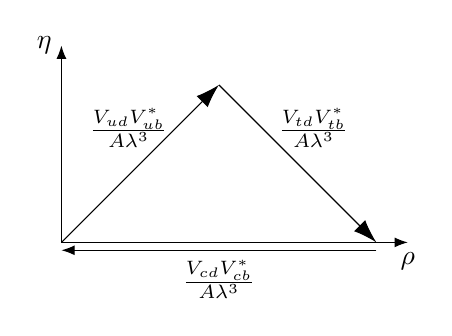
\begin{tikzpicture}
        \draw[-Latex] (0,0) -- (4.4,0) node[anchor=north] {$\rho$};
        \draw[-Latex] (0,0) -- (0,2.5) node[anchor=east] {$\eta$};
        \draw[-{Latex[length=3mm,width=2mm]}] (0,0) -- (2,2) node[anchor=north east,xshift=-15pt,yshift=-5pt] {$\frac{V_{ud}V_{ub}^*}{A\lambda^3}$};
        \draw[-{Latex[length=3mm,width=2mm]}] (2,2) node[anchor=north west,xshift=18pt,yshift=-5pt] {$\frac{V_{td}V_{tb}^*}{A\lambda^3}$} -- (4,0);
        \draw[-Latex] (4,-0.1) -- (0,-0.1) node[anchor=north,midway] {$\frac{V_{cd}V_{cb}^*}{A\lambda^3}$};
    \end{tikzpicture}
    \caption{\label{fig:unitang} The unitarity triangle from the Wolfenstein parameterisation in $(\rho,\eta)$ space.}
\end{figure}
The unitarity triangle can help describe many things in quark mixing, such as CP violation, through the length of its side and its angles. 
It can also be useful to define a unitarity circle through comparison of experiment and theory in CP-violating processes, and from these and others, many regions in the $(\rho,\eta)$ plane can be defined to interpret various constants and effects in quark mixing. 
\begin{figure}[H]
    \centering
    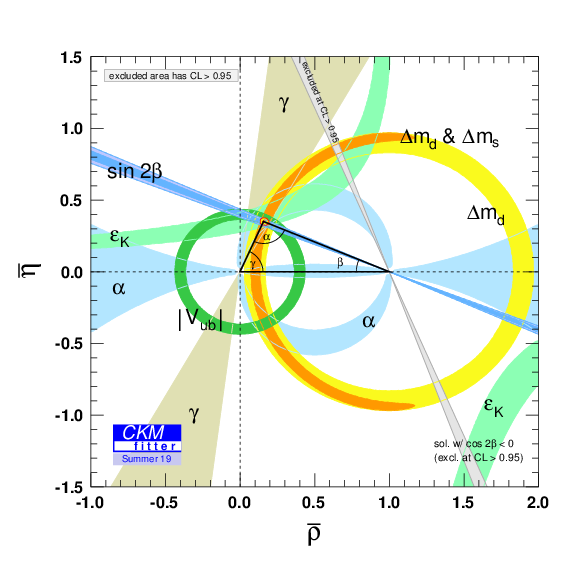
\includegraphics[scale=0.4,trim=0 20pt 0 50pt,clip]{rhoeta_large.png}
    \caption{\label{fig:ckmfitter} The global CKM fit in the $(\rho,\eta)$ plane, as of 13/01/20 \cite{ckm}.}
\end{figure}

\subsection{Flavour Physics and CP Violation}
\label{subsec:flavobs}
One of the big questions about the formulation of our universe is why is there an asymmetry between matter and anti-matter, known as Baryogenesis. 
Sakharov stated in 1967 three criteria that must have been fulfilled throughout the evolution of the Universe to create the current state of matter-antimatter asymmetry \cite{sak}. 
These are:
\begin{enumerate}
    \item Baryon Number Violation - this is theorised in sphalerons, though not yet confirmed experimentally \cite{sphal}. 
    \item C and CP Violation - this is present in the Standard Model, although not to the extent required. 
    \item A First Order Phase Transition in the early universe - this could have been possible in the Standard Model, but only for $m_h<60\,$GeV, whereas we now measure the Higgs mass to be $m_h=125.1\pm0.14\,$GeV.
\end{enumerate}
A significant focus of flavour physics is the study of CP violation - the violation of CP symmetry (the product of Charge and Parity symmetries) in the Standard Model.
CP symmetry was introduced as a candidate for the fundamental symmetry of Standard Model interactions after Parity violation was discovered in 1957 \cite{wu}.
Not long after, CP violation was also discovered, in 1964 in Kaon mixing \cite{cpv}.
CP violation has since been studied in the b-quark sector and recently discovered as well in the c-quark sector. 
The necessity of CP violation for the question of baryogenesis is apparent: if left-handed baryons interact differently to right-handed anti-baryons, then one of these can be more prominent than the other. 
Both the electromagnetic and strong forces appear to conserve CP, the weak force, however, through the chiral nature of its couplings, does not.
There are two ways for CP-violating interactions to occur through the weak force: through complex Yukawa couplings in the CKM matrix; and through complex Higgs parameters, such as those in the 2 Higgs Doublet Model to be discussed in section \ref{subsec:2hdm}.
There is also a question of whether CP violation can be found in the strong sector, but this will not be discussed here \cite{kane}.

Currently, there is a significant crux to the study of Sakharov's condition of CP violation: the amount of CP violation currently observed would not be enough to account for the large baryon asymmetry of the universe. 
This points toward physics beyond the Standard Model to add to the CP violation predicted and perhaps predict where to observe the CP violation needed in nature \cite{dono}. 
There are many proposals for Standard Model extensions which could bridge the gap between theory and experiment, although these extensions would require new particles to be observed to explain their phenomena, none of which have so far been observed. 

The $Z'$ boson is a common extension to the Standard Model, which in its simplest application behaves akin to the $Z^0$ boson but with a higher mass. 
There are many descriptions of the $Z'$ boson ranging from the introduction of a new U(1) gauge symmetry to the inclusion of string theory \cite{zp}. 
The consideration of a $Z'$ boson to flavour physics is to add extra coupling paths to scattering amplitudes which could better explain flavour observables. 
An example of how $Z'$ could modify Standard Model decays is given in Figure \ref{fig:bmes}.
\begin{figure}[H]
    \vspace{-20pt}
    \begin{equation}
        \Gamma_{\text{Exp}} = 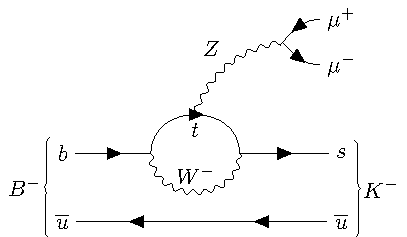
\includegraphics[scale=0.8,raise=-16pt]{../notes/bminus.pdf} + 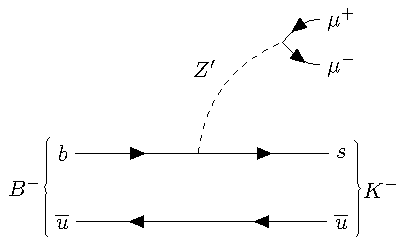
\includegraphics[scale=0.8,raise=-16pt]{../notes/bminusprime.pdf}
    \end{equation}
    \caption{\label{fig:bmes} Proposed $Z'$ extension to $\Gamma[B^-\to K^-\mu^+\mu^-]_{SM}$ (without higher-order terms).}
\end{figure}

It could also be possible that there is a fourth generation of fermions, perfectly replicating the first generation to higher masses as the second and third generations do. 
The presence of the fourth generation could add extra Feynman diagrams to decays, increasing the resulting decay amplitude. 
Another interesting implication of a fourth generation would be that the CKM matrix would now be a 4x4 matrix, which could see some alterations to flavour-changing interactions, even some additional complex terms where CP violation would arise. 
A key indicator on this extension is in the Higgs mechanism. 
\begin{figure}[H]
    \centering
    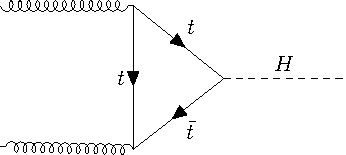
\includegraphics{../notes/higgs.pdf}
    \caption{\label{fig:higgs} Higgs boson production through the top quark loop.}
\end{figure}
The Higgs couples more strongly to heavier particles, so the top-Higgs vertex seen in Figure \ref{fig:higgs} should be replicated with the theoretical $t'$ and $b'$ quarks with increased amplitudes. 
However, when just considering the SM4 model, the new prediction of the Higgs scattering amplitude is far greater than that observed \cite{sm4}. 
It could be possible that the SM4 model is physical, but would also need another extension to resolve its issues, such as the Two Higgs Doublet Model discussed below \cite{shal}. 

%Whenever constructing new theories to extend the Standard Model, the inspiration can frequently come from a few specific cases of inconsistency. 
%However it is important to test these extensions across all observables which could involve the new processes.
%If the extension resolves issues with some observables while creating new ones with others, then it is of no use; only extensions which work across the whole spectrum of phenomena can be physical. 
%
\subsection{The Two Higgs Doublet Model of Type II}
\label{subsec:2hdm}
Previously in the Standard Model Higgs mechanism, to generate the masses of the weak gauge bosons and fermions, a single Higgs SU(2) doublet of complex scalar fields was introduced, as in Eq.\eqref{eq:doubscal}.
To form masses for both up- and down-type quarks and charged leptons, we introduced the hermitian conjugate doublet in Eq.\eqref{eq:highc}, otherwise the Higgs field would only give mass to the down-type quarks. 
Now two Higgs doublets can be postulated, of the general form
\begin{align}
    \label{eq:gdbl}
    \Phi_1 &= \begin{pmatrix} \phi_1 + i\phi_2 \\ \phi_0 + i\phi_3\end{pmatrix}, & \Phi_2 &= \begin{pmatrix} \phi_5+i\phi_6\\\phi_4+i\phi_7\end{pmatrix}.
\end{align}
These two doublets would have opposite hypercharge so one would couple to up-type quarks, and the other to down-type \cite{branco}. 
Each doublet would have its own VEV, with the quadrature addition of these two VEVs creating the value measured in experiment:
\begin{align}
    \label{eq:dbldbl}
    \Phi_1 &= \frac{1}{\sqrt{2}}\begin{pmatrix}0\\v_1\end{pmatrix}, & \Phi_2 &= \frac{1}{\sqrt{2}}\begin{pmatrix}v_2\\0\end{pmatrix}, & v_{SM}^2 &= v_1^2 + v_2^2.
\end{align}
Under this model, the masses of the three weak gauge bosons can still be generated in the same way, each eating one of the scalar fields. 
This time, however, there would be 5 residual scalar fields, and so, five Higgs fields should be found: three neutral Higgs - two scalar $H$ and $h$ (where $h$ is the SM Higgs particle) and one pseudoscalar $A$.
There will also be two charged Higgs $H^\pm$.
The introduction of these new particles requires searching for additional parameters to describe them: the masses of $H$, $A$, and $H^\pm$; the mixing angle between $h$ and $H$; and the VEV ratio $\tan\beta=v_2/v_1$ \cite{desc}.
The 2HDM potential can be written in its most general form as
\begin{align}
    \label{eq:HDMpot}
    \begin{split}
        V(\Phi_1,\Phi_2) =& m_{11}^2\Phi_1^\dagger\Phi_1 + m_{22}^2\Phi_2^\dagger\Phi_2 + m_{12}^2(\Phi_1^\dagger\Phi_2+\Phi_2^\dagger\Phi_1) + \frac{\lambda_1}{2}(\Phi_1^\dagger\Phi)^2 + \frac{\lambda_2}{2}(\Phi_2^\dagger\Phi_2)^2 \\
                                                        &+ \lambda_3\Phi_1^\dagger\Phi_1\Phi_2^\dagger\Phi_2 + \lambda_4\Phi_1^\dagger\Phi_2\Phi_2^\dagger\Phi_1 + \frac{\lambda_5}{2}\left[(\Phi_1^\dagger\Phi_2)^2+(\Phi_2^\dagger\Phi_1)^2\right].
    \end{split}
\end{align}
The two Higgs doublet model (2HDM) described above is the type II version, where $\Phi_1$ couples to up-type quarks and $\Phi_2$ couples to down-type quarks and charged leptons. 
There are other types of 2HDM where the two Higgs doublets couple in different ways, but the comforting sign from Type II is that it yields a similar expression for the Yukawa Lagrangian to the SM. 
This in turn yields a similar CKM matrix through which all flavour-changing interactions can be described. 
The addition of 4 new Higgs fields introduces new interactions, where the charged Higgs fields can replace $W$ fields in flavour-changing charged interactions, as well as additional neutral interactions between the neutral Higgs scalar and pseudoscalar fields \cite{branco}. 

The presence of charged Higgs fields presents the opportunity to bridge the gap between theory and experiment. 
The charged Higgs particles can mediate weak charged currents in the same way as $W^{\pm}$, and the additional contribution of $H^{\pm}$ to many weak-mediated decays could correct the Standard Model to predict these decay paths \cite{branco} more accurately. 
The important factors to determine whether these charged Higgs could be the answer to the inconsistencies are the relevant parameters from the 2HDM: the charged Higgs mass $m_{H^+}$, and the VEV ratio $\tan\beta$ \cite{desc}. 
Values of these parameters which align theory and observation can indicate where LHC experiments could probe for these theorised new particles. 
This study considers where regions of the 2HDM Type II parameters can align SM predictions with experiment, giving indication of where they could be found in nature if this model is to be a real extension of the Standard Model.

Finally, it is important to specify what makes the 2HDM Type II an interesting New Physics model to study. 
As hinted at when discussing the Sakharov criteria, one way of inducing CP violation would be through complex Higgs parameters. 
There are no such complex parameters in the Higgs sector of the Standard Model, however, as shown above, these are apparent in the 2HDM, and therefore we can introduce additional CP violation to possibly meet Sakharov's criterion. 
In addition to increased CP violation, the 2HDM also solves the problem of Sakharov's third criterion: under this model, a first order phase transition is present regardless of the value of the Higgs mass. 

\section{Probing the 2HDM Type II}
\label{sec:probe}
As mentioned previously, the 2HDM is easy to probe through the charged weak current, where interactions will gain additional pathways replacing a $W^{\pm}$ with a $H^{\pm}$. 
Studies of these new contributions have been done in the past, though it is interesting to revisit this now as new measurements are found, and SM calculations become more precise.
For flavour observables, a study of the most relevant decays for charged Higgs searches was found in \cite{desc}.
Here, we begin by following \cite{desc} closely to find the changes to their results in the last ten years, before moving on to further additions. 
The measurements and parameters used for these expressions is given in Tables \ref{tab:branches} and \ref{tab:params}.
\begin{table}[ht]
    \centering
    \begin{tabular}{c|ccc}
        \hline\hline
        Branching Ratios & Value & Unit & Reference \\
        \hline\hline
        $\Gamma[K^+\to\mu^+\nu_\mu]/\Gamma[\pi^+\to\mu^+\nu_\nu]$ & $1.337\pm0.003$ & & \cite{pdg}\\
        $\Gamma[\tau^+\to K^+\nu_\tau]/\Gamma[\tau^+\to\pi^+\nu_\tau]$ & $6.438\pm0.094$ & $10^{-2}$ & \cite{pdg} \\
        $\mathcal{B}r[B^+\to\mu^+\nu_\mu]$ & $5.3\pm2.2$ & $10^{-7}$ & \cite{bmu} \\
        $\mathcal{B}r[B^+\to\tau^+\nu_\tau]$ & $1.09\pm0.24$ & $10^{-4}$ & \cite{pdg} \\
        $\mathcal{B}r[D^+\to\mu^+\nu_\mu]$ & $3.82\pm0.33$ & $10^{-4}$ & \cite{pdg} \\
        $\mathcal{B}r[D_s^+\to\mu^+\nu_\mu]$ & $5.52\pm0.16$ & $10^{-3}$ & \cite{pdg} \\
        $\mathcal{B}r[D_s^+\to\tau^+\nu_\tau]$ & $5.48\pm0.23$ & $10^{-2}$ & \cite{pdg} \\
        $\mathcal{B}r[\bar{B}\to X_s\gamma]$ & $3.32\pm0.15$ & $10^{-4}$ & \cite{hflav,bmes} \\
        $\mathcal{B}r[\bar{B}\to X_c e\bar{\nu}]$ & $10.65\pm0.16$ & $10^{-2}$ & \cite{hflav,pdg} \\
        $\mathcal{B}r[\bar{B}\to X_ue\bar{\nu}]$ & $8.41\pm0.59$ & $10^{-4}$ & \cite{bxu} \\
        $\mathcal{B}r[B_d\to\mu^+\mu^-]$ & $1.4^{+1.6}_{-1.4}$ & $10^{-10}$ & \cite{pdg} \\
        $\mathcal{B}r[B_s\to\mu^+\mu^-]$ & $3.1\pm0.7$ & $10^{-9}$ & \cite{hflav} \\
        $\Delta m_d$ & $0.5064\pm0.0019$ & ps$^{-1}$ & \cite{hflav} \\ 
        $\Delta m_s$ & $17.757\pm0.021$ & ps$^{-1}$ & \cite{hflav} \\
        $\mathcal{R}(D)$ & $0.340\pm0.030$ & & \cite{hflav} \\
        $\mathcal{R}(D^*)$ & $0.298\pm0.014$ & & \cite{hflav} \\
        \hline\hline
    \end{tabular}
    \caption{\label{tab:branches}Branching ratios using in testing parameter space of 2HDM Type II. In the case of normalised ratios, values have been calculated using the constituent measurements taken from reference.}
\end{table}

\subsection{Leptonic Decays}
\label{subsec:lep}
In the Standard Model, the leptonic decay $M\to l\nu_l$, where $M$ is a charged meson, has a branching ratio of
\begin{equation}
    \label{eq:mlv}
    \mathcal{B}r[M\to l\nu_l]_{\text{SM}} = \frac{G_F^2m_Mm_l^2}{8\pi}\left(1-\frac{m_l^2}{m_M^2}\right)^2 |V_{q_uq_d}|^2f_M^2\tau_M(1+\delta_{EM}^{Ml2}),
\end{equation}
where $q_u$ and $q_d$ represent the up- and down-like quarks of the meson, $V_{q_uq_d}$ the CKM element, $f_M$ the $M$ meson's decay constant, and $G_F$ is the Fermi constant, defined as
\begin{align}
    G_F &= \frac{g_2^2\sqrt{2}}{8M_W^2} \approx 1.166\times10^{-5}\,\text{GeV}^{-2}.
\end{align}
$\delta_{EM}^{Ml2}$ is a corrective factor for electromagnetic radiative corrections. 
For $\pi$ and $K$ mesons, the effect is around 2-3\% and around 1\% for $D$ mesons.
For B meson phenomena, the effect is approximated to 0. 
\begin{figure}[ht]
    \centering
    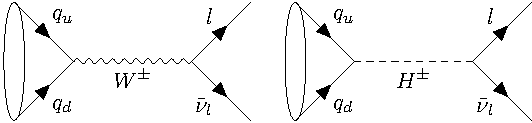
\includegraphics[width=0.8\textwidth]{mesons.pdf}
    \caption{\label{fig:mesons}$W^\pm$ and $H^\pm$ pathways for the leptonic decay of a meson (before higher-order terms).}
\end{figure}
For the light mesons, kaons and pions, it is easier to determine the ratio of their decay constants $f_K/f_\pi$ than the individual values.
Thus, it is then easier to consider the ratio of their branching fractions as well. 
In the Standard Model, 
\begin{equation}
    \label{eq:kpi}
    \frac{\Gamma[K\to\mu\nu]_{\text{SM}}}{\Gamma[\pi\to\mu\nu]_{\text{SM}}} = \frac{m_K}{m_\pi}\left(\frac{1-m_l^2/m_K^2}{1-m_l^2/m_\pi^2}\right)^2 \bigg|\frac{V_{us}}{V_{ud}}\bigg|^2\left(\frac{f_K}{f_\pi}\right)^2(1+\delta^{Kl2/\pi l2}_{EM}).
\end{equation}
It is also worth considering the ratio of tau decays of kaons to pions:
\begin{equation}
    \label{ep:tkpi}
    \frac{\Gamma[\tau\to K\nu]_{\text{SM}}}{\Gamma[\tau\to\pi\nu]_{\text{SM}}} = \left(\frac{1-m_K^2/m_\tau^2}{1-m_\pi^2/m_\tau^2}\right)^2\bigg|\frac{V_{us}}{V_{ud}}\bigg|^2\left(\frac{f_K}{f_\pi}\right)^2(1+\delta_{EM}^{\tau K2/\tau\pi2}).
\end{equation}

These SM branching values will take alterations from the two Higgs doublet model of the form
\begin{equation}
    \label{eq:mesrh}
    \mathcal{B}r[M\to l\nu] = \mathcal{B}r[M\to l\nu]_{\text{SM}}(1+r_H)^2,
\end{equation}
where $r_H$ is the corrective factor of the two Higgs doublet model:
\begin{align}
    \label{eq:rh}
    r_H &= \left(\frac{m_{q_u}-m_{q_d}\tan^2\beta}{m_{q_u}+m_{q_d}}\right)\left(\frac{m_M}{m_{H^+}}\right)^2.
\end{align}
It can still be possible through this method for some leptonic decays to have agreement between the SM predictions and experiment, where $r_H = 0,-2$.
$r_H=0$ is known as the decoupling solution which can be found as $m_{H^+}$ approaches infinity; $r_H=-2$, the fine-tuned solution, is obtained from a linear relationship between $m_{H^+}$ and $\tan\beta$, which will be dependent of the masses of the meson and its constituent quarks, so will vary between mesons. 

\subsection{Mass mixing}
\label{subsec:mix}
Neutral B meson mixing is a common study in flavour physics, due to the strong dependence on the heavy $W$ exchange. 
\begin{figure}[ht]
    \centering
    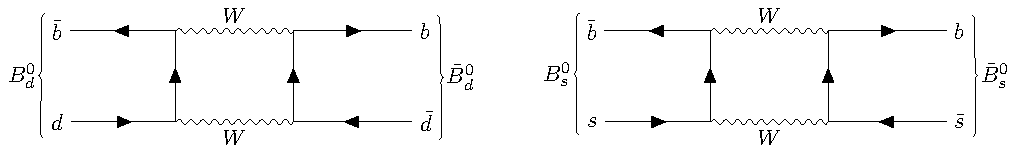
\includegraphics[scale=0.95,trim=12em 45em 10em 12em]{bmix.pdf}
    \caption{\label{fig:bmix} Examples of the box diagrams detailing $B_d$ and $B_s$ meson mixing.}
\end{figure}
A key observable in the study of B-mixing is the mass difference $\Delta m_q$ between the two mass eigenstates $\Delta m_q = M_H^q - M_L^q$, where `$H$' denotes the `heavy' eigenstate and `$L$' denotes the `light'. 
A thorough description of this process can be found, for example, in \cite{mix15}.
In the 2HDM, the mass difference receives two additional contributions from box diagrams using the heavy charged Higgs in place of both $W$s or one $W$. 
For $B_q$, where $q=d,s$, this results (to Leading Order) in:
\begin{align}
    \Delta m_q &= \frac{G_F^2}{6\pi^2}(V_{tq}V_{tb}^*)^2\hat{\eta}_Bm_Bm_W^2f_{B_q}^2B_{B_q}(S_{WW}+2S_{WH}+S_{HH}), \\
    S_{WW} &= x_{tW}\left(\frac14+\frac{9}{4(1-x_{tW})}-\frac{3}{2(1-x_{tW})^2}-\frac{3x_{tW}^2\ln(x_{tW})}{2(1-x_{tW})^3}\right), \\
    S_{HH} &= \frac{x_{tH}x_{tW}}{4\tan^4\beta}\left(\frac{1+x_{tH}}{(1-x_{tH})^2}+\frac{2x_{tH}\ln(x_{tH})}{(1-x_{tH})^3}\right),\\
    2S_{WH} &= \frac{x_{tH}x_{tW}}{4\tan^2\beta}\left(\frac{(2x_{tW}-8x_{tH})\ln(x_{tH})}{(1-x_{tH})^2(x_{tH}-x_{tW})}+\frac{6x_{tW}\ln(x_{tW})}{(1-x_{tW})^2(x_{tH}-x_{tW})}-\frac{8-2x_{tW}}{(1-x_{tH})(1-x_{tW})}\right).
\end{align}
where $x_{ij} = m_i^2/m_j^2$, and $S_{xy}$ describes the internal bosonic lines for the two bosons $x,y \in H^\pm,W^\pm$.
The current SM predictions for the mass differences are stated in \cite{bmix} as
\begin{align}
    \Delta m^{\text{SM}}_d &= \left(0.533^{+0.022}_{-0.036}\right)ps^{-1} = \left(1.05^{+0.04}_{-0.07}\right)\Delta m_d^{\text{exp}}, \\
    \Delta m^{\text{SM}}_s &= \left(18.4^{+0.7}_{-1.2}\right)ps^{-1} = \left(1.04^{+0.04}_{-0.07}\right)\Delta m_s^{\text{exp}}.
\end{align}

\subsection{Radiative decay}
\label{subsec:rad}
The radiative decay $b\to s\gamma$ occurs through the flavour-changing neutral currents of penguin diagrams.
The Standard Model calculations of $\bar{B}\to X_s\gamma$ have been performed up to Next-to-Next Leading Order (NNLO), which yields a complicated expression, so the result is parameterised in line with \cite{desc,susy}.
\begin{figure}[H]
    \centering
    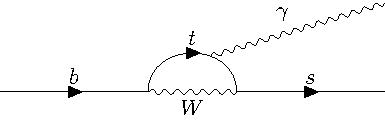
\includegraphics[width=\textwidth]{bsgam.pdf}
    \caption{\label{fig:bsgam} One-loop penguin diagrams for $b\to s\gamma$ decay.}
\end{figure}
Similarly to B meson mixing, W can be substituted for a charged Higgs in all the relevant penguin diagrams, giving extra contributions again to the theory. 
The 2HDM corrections given by these additional contributions are calculated to NLO in \cite{susy}, so the SM parameters must be limited to NLO.
The branching ratio of $\bar{B}\to X_s\gamma$ is given by
\begin{equation}
    \label{eq:xsgam}
    \mathcal{B}r[\bar{B}\to X_s\gamma] = \mathcal{B}r[\bar{B}\to X_cl\bar{\nu}] \bigg|\frac{V_{ts}^*V_{tb}}{V_{cb}}\bigg|^2 \frac{6\alpha_{\text{EM}}}{\pi C}(P+N),
\end{equation}
where we calculate using the branching ratio of $\bar{B}\to X_cl\bar{\nu}$ to cancel out the high uncertainties from quark mass terms.
Here, $P$ represents the perturbative leading contribution in the heavy quark expansion, and $N$ the non-perturbative higher-order contributions of the heavy quark expansion.
$P$ and $N$ are parameterised in \cite{desc,susy} as 
\begin{equation}
    \label{eq:pplsn}
    P+N = (C^{\text{eff},(0)}_{7,SM}+B\Delta C_{7,H^+}^{\text{eff},(0)})^2+A,
\end{equation}
where $A$ and $B$ are functions defined in \cite{desc}, $C_{7,SM}^{\text{eff},(0)}$ is one of the Wilson coefficients of the effective Hamiltonian in the SM, and $\Delta C_{7,H^+}^{\text{eff},(0)}$ holds the charged Higgs contributions to the SM Wilson coefficient. 
Although these expressions are calculated to NLO, in calculating the above Wilson coefficients, we choose a renormalisation scheme $\mu_b$ such that we recover the results of the NNLO calculation. 

In Eq.\eqref{eq:xsgam}, $C$ is the non-perturbative phase-space normalisation factor for the difference between the charmed semileptonic branching ratio and $\bar{B}\to X_s\gamma$. 
From \cite{bmes}, it is defined as 
\begin{align}
    \label{eq:phasespace}
    C &= \bigg|\frac{V_{ub}}{V_{cb}}\bigg|^2\frac{\Gamma(\bar{B}\to X_ce\bar{\nu})}{\Gamma(\bar{B}\to X_ue\bar{\nu})}.
\end{align}
This factor is important to cancel out the charm contribution we included earlier in $\mathcal{B}r[\bar{B}\to X_cl\bar{\nu}]$ to return us to the charmless state we consider.
For these calculations, we follow the parameterisation of this process laid out in Appendix B of \cite{desc}.

\subsection{Updating The 2HDM Constraints}
\label{subsec:fit}
\begin{table}
    \centering
    \begin{tabular}{c|ccc}
        \hline\hline
        Input & Value & Unit & Reference \\
        \hline\hline
        \multicolumn{4}{c}{\bfseries Decay Constants} \\
        \hline\hline
        $f_K/f_\pi$ & $1.1932\pm0.0019$ & & \cite{pdg}\\
        $f_B$ & $190\pm1.3$ & MeV & \cite{flag} \\
        $f_{B_s}$ & $230\pm1.3$ & MeV & \cite{flag} \\
        $f_D$ & $212\pm0.7$ & MeV & \cite{flag} \\
        $f_{D_s}$ & $249.9\pm0.5$ & MeV & \cite{flag} \\
        \hline\hline
        \multicolumn{4}{c}{\bfseries Radiative corrections} \\
        \hline\hline
        $\delta^{Kl2/\pi l2}_{EM}$ & $-0.0069\pm0.0017$ & & \cite{pdg} \\
        $\delta^{\tau K2/\tau\pi 2}_{EM}$ & $0.003$ & & \cite{desc} \\
        \hline\hline
        \multicolumn{4}{c}{\bfseries B meson mixing} \\
        \hline\hline
        $f^2_{B_d}B_{B_d}$ & $0.0305\pm0.0011$ & GeV$^2$ & \cite{bmix} \\
        $f^2_{B_s}B_{B_s}$ & $0.0452\pm0.0014$ & GeV$^2$ & \cite{bmix} \\
        $\hat{\eta}_B$ & $0.838606$ & & \cite{alex} \\
        \hline\hline
        \multicolumn{4}{c}{\bfseries $\mathbf{b\to s\gamma}$ parameters} \\
        \hline\hline
        $m_t^{pole}$ & $173.1\pm0.9$ & GeV & \cite{pdg} \\
        $\alpha_S(m_Z)$ & $0.1179\pm0.001$ & & \cite{pdg} \\
        $\mu_b$ & $1.095$ & GeV & \\
        \hline\hline
    \end{tabular}
    \caption{\label{tab:params} Parameters used in the 2HDM fits for decays outlined in Section \ref{sec:probe}.}
\end{table}
Before adding to the fit performed in \cite{desc}, we check that we can replicate their results from 2009 and update this with the most recent input values. 
All processes mentioned above were used to test the constraints on the 2HDM parameters $m_{H^+}$ and $\tan\beta$. 
The 2HDM-extended branching ratios were tested in $(m_{H^+},\tan\beta)$ parameter space to search for regions where a charged Higgs would be allowed by nature. 
The individual constraints found for leptonic decays, B meson mixing, and the radiative $b\to s\gamma$ decay are shown in Figure \ref{fig:indies} in a log-log scale.
After the constraints on the 2HDM for each individual process were found, they were combined for a global fit shown in Figure \ref{subfig:glob11} (again in a log-log scale), yielding an overall allowed region in $(m_{H^+},\tan\beta)$ space. 

For each constraint, a scan was performed to $2\sigma$ to find regions where the parameter space is not excluded at this level. 
A $\chi^2$ fit was then performed to constrain these regions to where $\Delta\chi^2$ corresponded to 95\% CL exclusion, such that each region shown in these Figures shows what is not excluded to 95\% CL.
For the combined fit, we also show the $1\sigma$ confidence region. 

To test the validity of these results, we also show what our calculations produce for 2009 inputs, as done in \cite{desc}.
This fit is shown in Figure \ref{subfig:glob08}, where it is seen to replicate the previous results, finding $m_{H^+} > 316\,$GeV at 95\% CL.
\begin{figure}[ht]
    \vspace{-12pt}
    \centering
    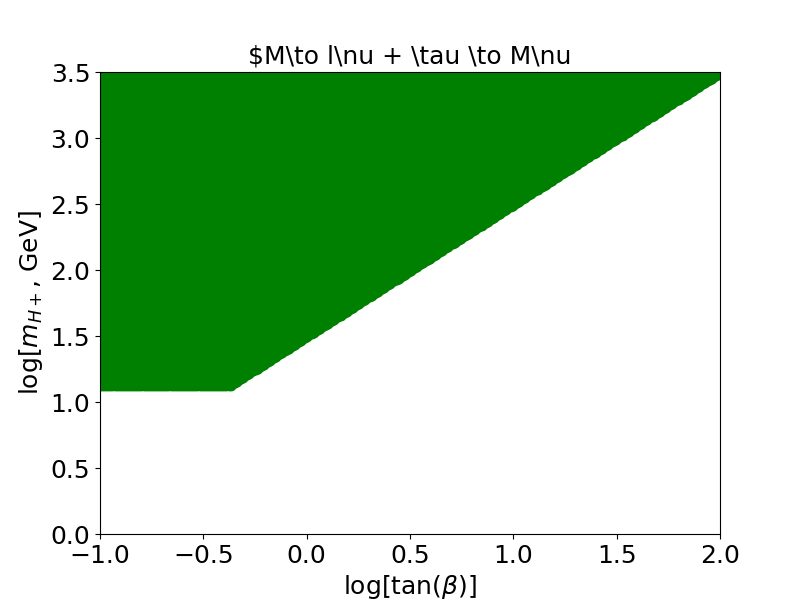
\includegraphics[width=0.49\textwidth]{indy/leps.png}
    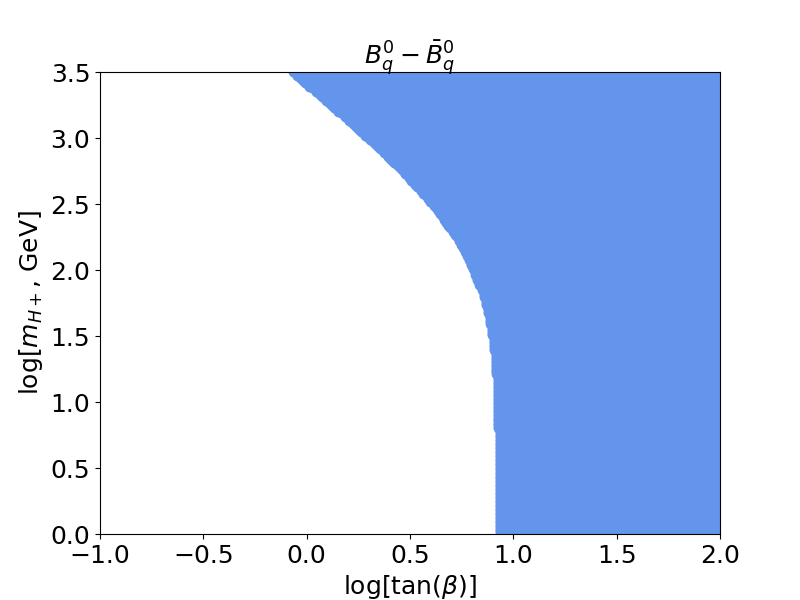
\includegraphics[width=0.49\textwidth]{indy/bmix.png}
    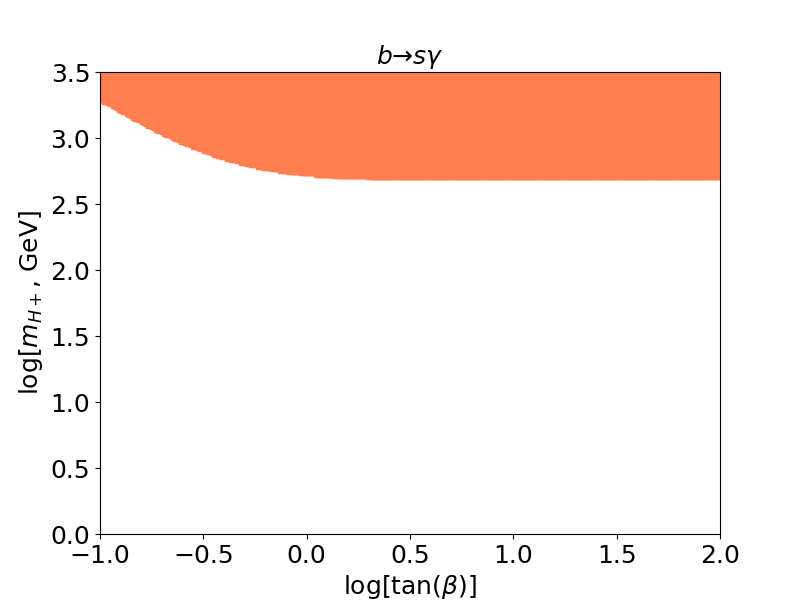
\includegraphics[width=0.49\textwidth]{indy/bsgamma.png}
    \caption{\label{fig:indies}Constraints of $(m_{H^+},\tan\beta)$ space from leptonic decays (top left), $B_d$ and $B_s$ mixing (top right), and the radiative $b\to s\gamma$ decay (bottom). The leptonic decays used were $B^+\to\tau^+\nu$, $B^+\to\mu^+\nu$, $D^+\to\mu^+\nu$, $D_s^+\to\mu^+\nu$, $D_s^+\to\tau^+\nu$, and the ratios $K\to\mu\nu/\pi\to\mu\nu$ and $\tau\to K\nu/\tau\to\pi\nu$. 
        The solid black vertical line (top right) shows $\tan\beta=m_t/m_b$, as for $\tan\beta$ much greater than this, the formulae for B mixing become invalid. 
    Each region shows what is not excluded to 95\% CL, as discussed in the text.}
\end{figure}
The 2HDM is generally taken to be a decoupling theory. 
That is, taking the limit $m_{H^+} \to \infty$ should recover the Standard Model picture of physics.
For as far as we scan here, this is reinforced in our results, such that there is no upper bound on $m_{H^+}$. 
We also see that for the combined fit, $\tan\beta$ will extend both to smaller and larger values as $m_{H^+}\to\infty$, such that there is no definitive constraint on $\tan\beta$. 
There is, however, a clear indication of a minimum allowed value for $m_{H^+}$, found here as
\begin{align}
    \label{eq:const}
    m_{H^+} >
    \begin{split}
         &\; 480 \;\text{GeV},\quad 95\% \text{ CL},\\
         &\; 750 \;\text{GeV},\quad 1\sigma.
    \end{split}
\end{align}
\begin{figure}[ht]
    \centering
    \begin{subfigure}[b]{0.48\textwidth}
        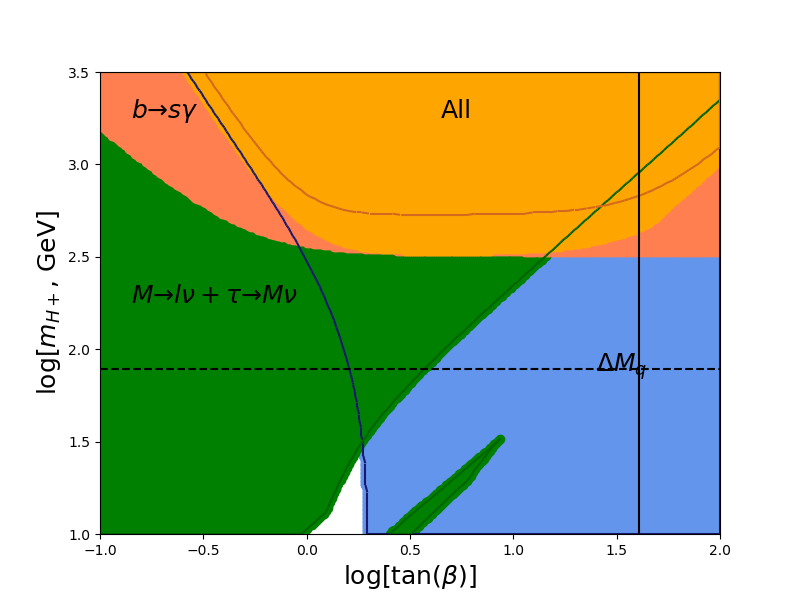
\includegraphics[width=\textwidth]{global08.png}
        \caption{\label{subfig:glob08}First global fit with 2009 inputs.}
    \end{subfigure}
    \begin{subfigure}[b]{0.48\textwidth}
        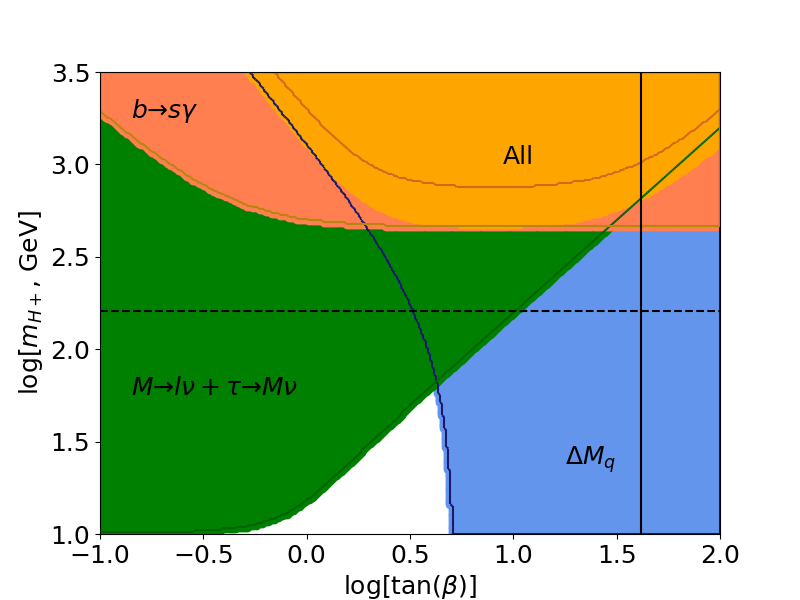
\includegraphics[width=\textwidth]{../global/global_test_min.png}
        \caption{\label{subfig:glob11}First global fit with 2020 inputs.}
    \end{subfigure}
    \caption{\label{fig:glob1} First global fit of constraints on $m_{H^+}$ and $\tan\beta$ from observables considered in \cite{desc}. 
    Each region shows what is not excluded for the relevant observables to 95\% CL as discussed in the text, then the line within the orange region for all observables marks out the $1\sigma$ confidence area. 
    The solid black vertical line shows $\tan\beta=m_t/m_b$, as for $\tan\beta$ much greater than this, the formulae for B mixing are invalid. 
    The dashed horizontal line marks the limit from direct searches, at $m_{H^+}>160\,$GeV \cite{dirhp}.}
\end{figure}

\subsection{New Observables}
\label{sec:rdbmu}
Having found agreement with the fit in \cite{desc}, and updating this with new inputs, we move on to new observables not yet considered. 
There are some observables discussed in previous works that they did not include in their fit that we discuss here, as well as some that have had improved work in experiment and theory over the last 10 years. 

\subsubsection{$B^+\to\mu^+\nu$}
The heavily CKM- and helicity-suppressed leptonic decay was recently measured by the Belle collaboration \cite{bmu}, and can be added to the fit using the theory for leptonic decays in Section \ref{subsec:lep} for the first time to either reinforce the structure of the leptonic decay region in Figure \ref{fig:indies} or to show new sensitivity.
This decay is now included in the leptonic fit in Figure \ref{fig:indies}, and does not constrain the model any more than the other leptonic decays. 

\subsubsection{$B_{d,s}\to\mu^+\mu^-$}
These decays can be particularly sensitive to scalar operator effects in new physics, and as such, are excellent probes for the 2HDM and the additional effects this could have. 
In the 2HDM, this process is given by (for $q=d,s$)
\begin{align}
    \begin{split}
        \mathcal{B}r[B_{q}\to\mu^+\mu^-] = &\frac{G^4_FM_W^4s_W^4}{32\pi^5}|V_{tb}^*V_{tq}|^2f(r^2,r^2)M_{B_q}f_{B_q}^2(4m_\mu^2)\tau_{B_q} \\
                                           &\times\Bigg\{\bigg|\frac{M_{B_q}^2(C_P^*-C_P^{'*})}{(m_q+m_b)(2m_\mu)}-(C_{10}^*-C_{10}^{'*})\bigg|^2 +\bigg|\frac{M_{B_q}^2(C_S^{'*}-C_S^*)}{(m_q+m_b)(2m_\mu)}\bigg|^2\left[1-4r^2\right]\Bigg\},
    \end{split}
\end{align}
where we follow \cite{criv} for the expressions of the relevant Wilson coefficients and the definitions of $f(x,y)$ and $r$, and $s_W=\sin\theta_W$ is the weak mixing angle. 
\begin{figure}[H]
    \centering
    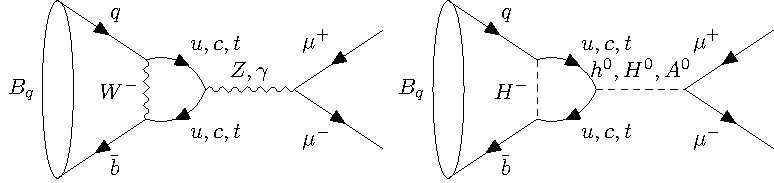
\includegraphics[width=\textwidth]{bsmu.pdf}
    \caption{\label{fig:bspeng}Examples of penguin contributions to $B_q\to\mu^+\mu^-$ operators.}
\end{figure}
Previous works, see \cite{lrgtb}, have focused on studying these processes in the large $\tan\beta$ limit ($\tan\beta\gg\sqrt{\frac{m_t}{m_b}}$) where the Yukawa coupling to $b$ quarks is large and there can large effects on B mesons. 
Working in the large $\tan\beta$ limit is also useful as it reduces the number of 2HDM parameters that this process will depend on. 
However, in this work, we choose to work with the general expressions, as given by \cite{criv}, to work with our fit across the whole parameter space we study. 
Using these general expressions, however, introduces new variables, primarily in the expressions for the trilinear Higgs couplings which we take from \cite{trilin}.
These new variables are: the masses of the neutral $h^0,H^0$, the mixing angle $\alpha$, and the 2HDM potential parameter $M=\frac{m_{12}^2}{\sin\beta\cos\beta}$ (see Eq. \ref{eq:HDMpot}). 
These new parameters can all be varied along with $m_{H^+}$ and $\tan\beta$ in a higher-dimensional fit, although it is simpler to fix some of these at set values. 

When working in the 2HDM, it is usually assumed that we are working in the \emph{alignment limit}, where the lighter neutral Higgs $h^0$ is taken to be the observed Higgs, and the mixing angles are aligned such that $\cos(\beta-\alpha) \approx 0$. 
Using this limit therefore allows us to fix $\alpha$ and $m_{h^0}$, leaving two additional parameters.
Scanning in ($m_{H^+},\tan\beta$) space, as for other observables, for fixed values of $M$ and $m_{H^0}$ across a range based on the work in \cite{trilin} and the direct searches for $H^0$ in \cite{h0search}, we find that $M$ bears no significance on the constraints, $\chi^2_{min}$, or p-values of the fit.
We therefore fix $M=750\,$GeV as the median value in the range considered.
The value of $m_{H^0}$, however, does change the scan across the range chosen. 
We show here the impact of different values of $m_{H^0}$ on the allowed region of parameter space at the extremities and the middle of our range. 
\begin{figure}[ht]
    \centering
    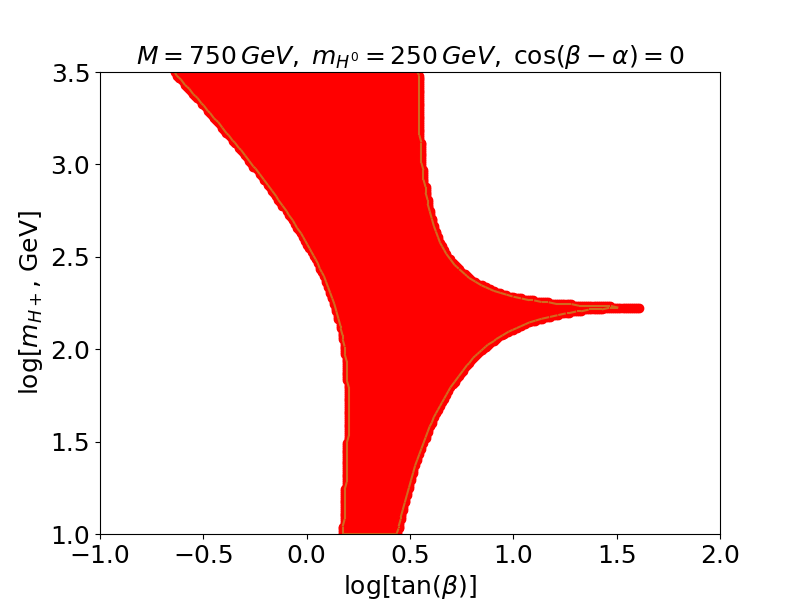
\includegraphics[width=0.32\textwidth]{bmu1.png}
    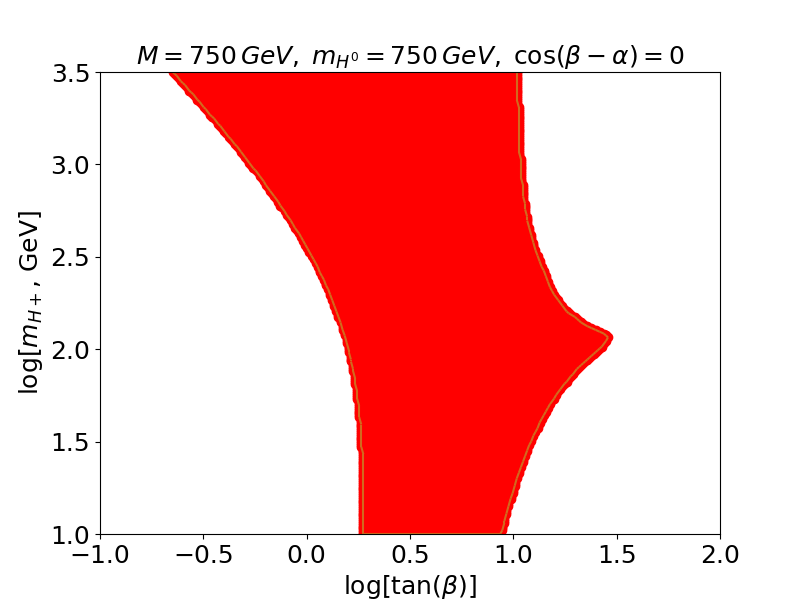
\includegraphics[width=0.32\textwidth]{bmu2.png}
    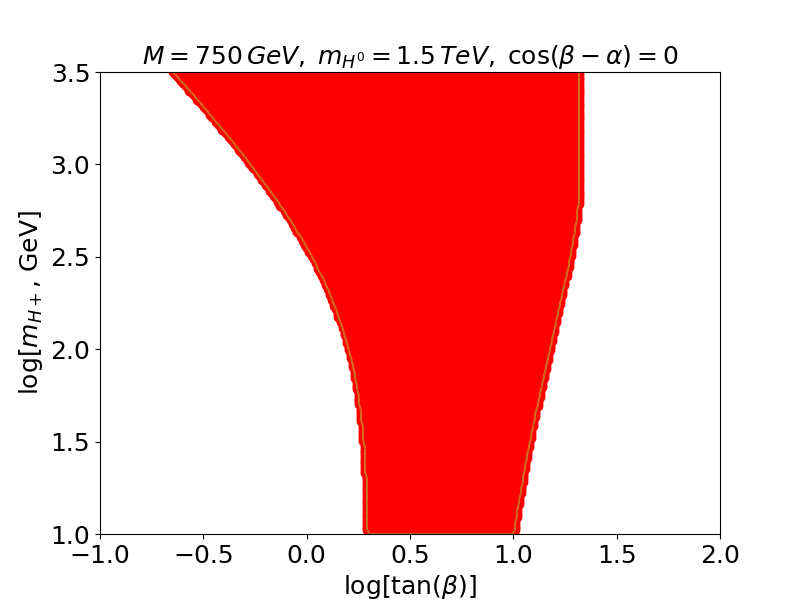
\includegraphics[width=0.32\textwidth]{bmu3.png}
    \caption{\label{fig:bmu}Constraints on ($m_{H^+},\tan\beta$) space from $B_{s,d}\to\mu^+\mu^-$ decays, for $M=750\,$GeV, $\cos(\beta-\alpha)=0$ and varying fixed values of $m_{H^0}$ - $250\,$GeV (left), $750\,$GeV (center), $1.5\,$TeV (right).
        The red region in each plot indicates allowed parameter space after exclusion at 95\% CL.}
\end{figure}
We see that there is no specific constraint on $m_{H^+}$ as we move towards $\infty$, and these processes by themselves do not give a minimum value of $m_{H^+}$. 
We do however now see more significant bounds on $\tan\beta$ than we had previously. 
The extent of the constraint on $\tan\beta$ depends on $m_{H^+}$ as seen in Figure \ref{fig:bmu}.
When added to the global constraints, this will restrict larger $\tan\beta$ values depending on $m_{H^0}$.
Testing across the range of values for $m_{H^0}$, we find that using $m_{H^0}=1.5\,$TeV minimises $\chi^2$ and maximises the p-value of our fit; see Section \ref{sec:discuss} and Table \ref{tab:pval1} for details of this fit.
Further analysis into this three-dimensional parameter space introduced here will be discussed in Section \ref{subsec:oblique}.

\subsubsection{$\mathcal{R}(D)$ and $\mathcal{R}(D^{(*)})$}
\begin{figure}[H]
    \centering
    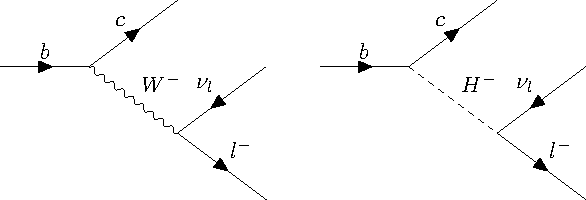
\includegraphics[width=0.8\textwidth]{bclnu.pdf}
    \caption{\label{fig:bclnu}Tree level decay diagrams for the $b\to cl\nu$ transitions in $B\to D^{(*)}l\nu$.}
\end{figure}
These semileptonic decay ratios, defined as
\begin{align}
    \mathcal{R}(D^{(*)}) &=\frac{\mathcal{B}r[B\to D^{(*)}\tau\nu]}{\mathcal{B}r[B\to D^{(*)}l\nu]},
\end{align}
are well-studied anomalies in the Standard Model, deviating from the Standard Model predictions by $1.4\sigma$ and $2.5\sigma$ respectively \cite{pdg}. 
Due to these deviations, these ratios seem well-suited for testing constraints on new physics models. 
In \cite{desc}, a 2HDM parameterisation of $\mathcal{R}(D)$ was discussed and was said to align similarly with the leptonic constraints, however, they did not discuss $\mathcal{R}(D^*)$. 
\begin{figure}[ht]
    \centering
    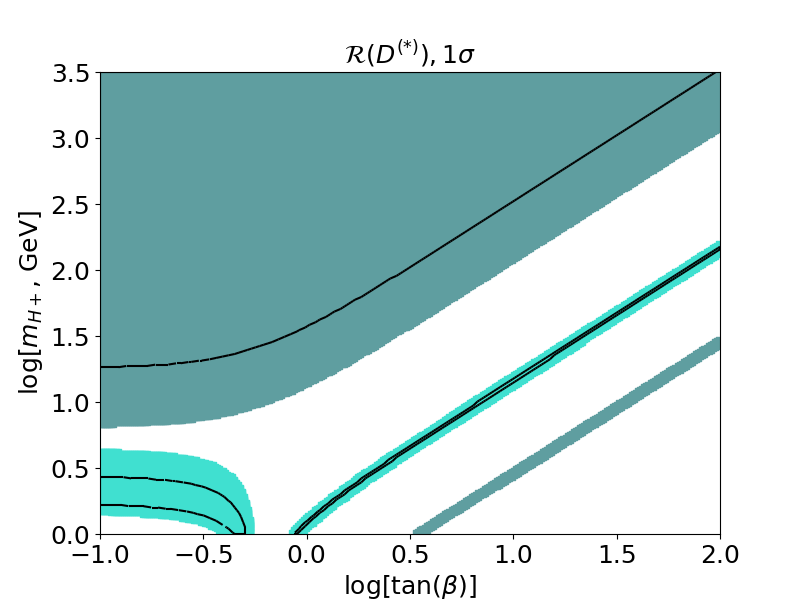
\includegraphics[width=0.49\textwidth]{rd_both196sig.png}
    \caption{\label{fig:rds}Constraint on ($m_{H^+},\tan\beta$) space from $\mathcal{R}(D)$ (blue) and $\mathcal{R}(D^*)$ (turquoise) using a $2\sigma$ scan, then $\chi^2$ fitting as described in the text. 
    The black lines for each region outlines the 95\% CL region and the blue lines outline the $1\sigma$ confidence region.}
\end{figure}
We follow the expressions for $\mathcal{R}(D^{(*)})$ in the 2HDM found in Section III of \cite{rds} and perform a scan as before on these observables. 
Historically, the 2HDM has struggled to fit both these ratios simultaneously, and it may be a killer argument for this model if no resolution to this can be found. 
So far we have implemented $2\sigma$ scans, and at this level, $\mathcal{R}(D^*)$ excludes the 2HDM.
However, exclusion at this level only means that the 2HDM performs no better than the Standard Model for this observable. 
We therefore move forward with two approaches to work through this discrepancy: we continue to fit all observables at the $2\sigma$ level, excluding $\mathcal{R}(D^*)$ as an anomaly as it is in the Standard Model; and we also scan to higher $\sigma$, as $\mathcal{R}(D^*)$ may then agree with the fit to this level, leaving room for further discussion on resolving its deviation.
\begin{figure}[ht]
    \centering
    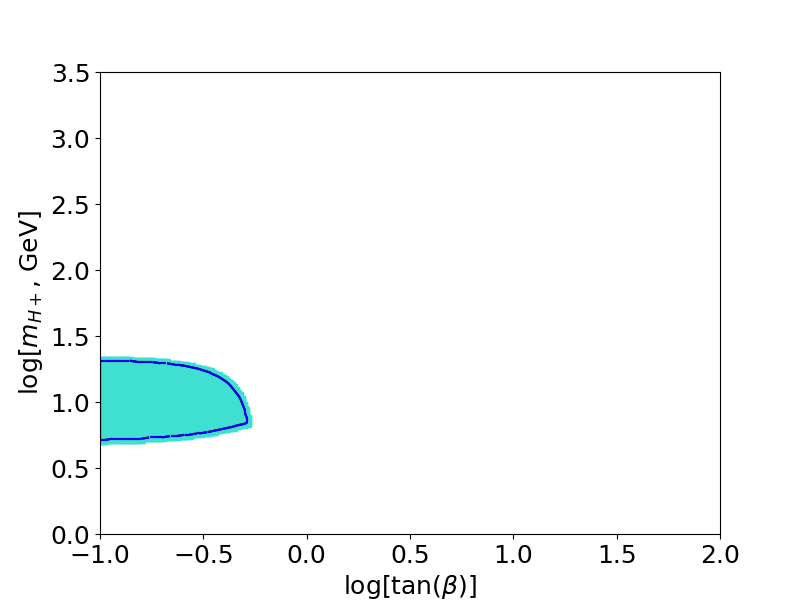
\includegraphics[width=0.49\textwidth]{rd_both25sig.png}
    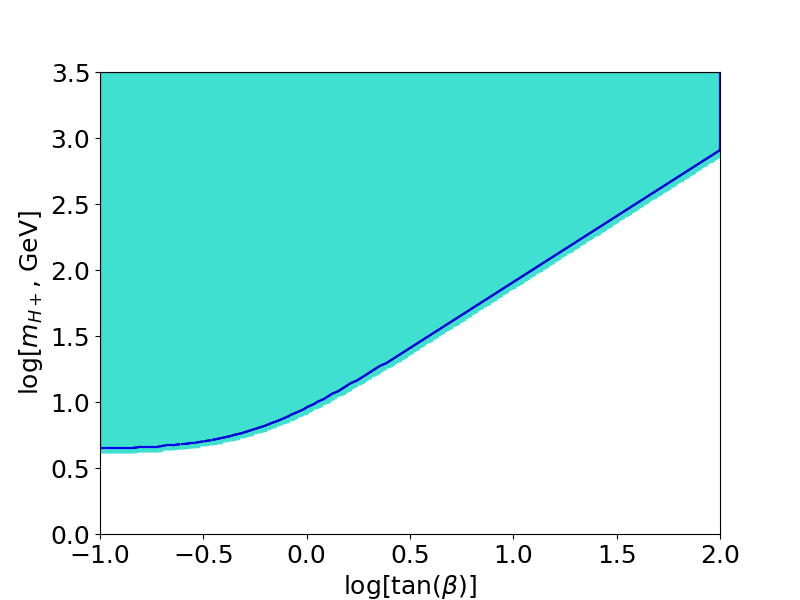
\includegraphics[width=0.49\textwidth]{rd_both3sig.png}
    \caption{\label{fig:rd3sig}Constraint on ($m_{H^+},\tan\beta$) space from $\mathcal{R}(D)$ and $\mathcal{R}(D^*)$ from a $2.5\sigma$ scan (left) and $3\sigma$ scan (right). 
    The turquoise region shows what is not excluded for the joint fit of these two observables from the scan, and the blue line indicates the outline of the 95\% CL region.}
\end{figure}
In Figure \ref{fig:rd3sig}, it is shown that the joint constraint from $\mathcal{R}(D)$ and $\mathcal{R}(D^*)$ aligns well with that of the leptonic decays in Figure \ref{fig:indies} when we now scan at $3\sigma$, but the 2HDM does fit this slightly worse than the Standard Model, as $\mathcal{R}(D^*)$ will still lead to an exclusion at $2.5\sigma$. 
We test our fit with $\mathcal{R}(D^*)$ included as an anomaly at $2\sigma$, and also include it as in Figure \ref{fig:rd3sig} to a $3\sigma$ scan. 
The statistical significance of these approaches are found in Tables \ref{tab:pval1} and \ref{tab:pval2}.

\subsection{SM4 with Two Higgs Doublet Model}
As discussed in Section \ref{subsec:flavobs}, a fourth generation of fermions can be proposed as a way of inducing more CP violation, but the SM4 model alone has been excluded. 
One proposal to still include a fourth generation is to combine this with the 2HDM. 
Traditionally in the 2HDM, we take the alignment limit to replicate the observed Higgs particle in the lighter neutral Higgs $h$ of the 2HDM.
This also follows from measurements of the coupling strengths of the Higgs sector, which agree with the SM predictions within $1\sigma$ \cite{couple}.

There is, however, an alternate treatment to this data. 
LHC measurements may measure the magnitudes of the couplings to closely align with the Standard Model, but they cannot necessarily determine the phase of the coupling. 
Defining $\kappa_i$ as the ratio of the 2HDM Higgs coupling to particles $ii$ to the SM coupling, we therefore can propose a scenario in which 
\begin{align}
    \kappa_{W,Z} &= 1, & \kappa_u &= 1, & \kappa_{d,l} &= -1,
\end{align}
where $u$ denotes up-type quarks, $d$ down-type quarks, and $l$ the charged leptons.
In this scenario, the common argument for the exclusion of the SM4 model that the gluon fusion Higgs production would be enhanced by a factor 9 over the Standard Model would no longer be valid as the new quark contributions approximately cancel each other and we approximately recover the SM result.
This is known as the \emph{wrong sign limit} (for a review, see e.g. \cite{wrong1,wrong2}).
Within the 2HDM Type II, this limit can be written with the relationship
\begin{align}
    \label{eq:wrongsign}
    \cos(\beta-\alpha) = \sin(2\beta), \text{ or equivalently when} \tan\beta\gg2,\; \cos(\beta-\alpha) = 2\cot\beta.
\end{align}
In this work, we consider the wrong sign limit in the 2HDM only, as an indication of its validity for use in future works considering the 2HDM fit in the framework of SM4. 
Moving forward, in addition to working in the alignment limit as discussed previously, we consider the exact wrong sign limit from Eq. \ref{eq:wrongsign}, and the use of numerical constraints on $\tan(\beta)$ provided from collaboration of the fit with \cite{oliver}.
The only observable that is dependent on the limit we choose for the Higgs couplings so far is $B_q\to\mu^+\mu^-$, so we now look to other observables that can also compare the alignment and wrong sign limits.

\subsection{The Global Fit with Oblique Parameters}
\label{subsec:oblique}
\begin{figure}[ht]
    \centering
    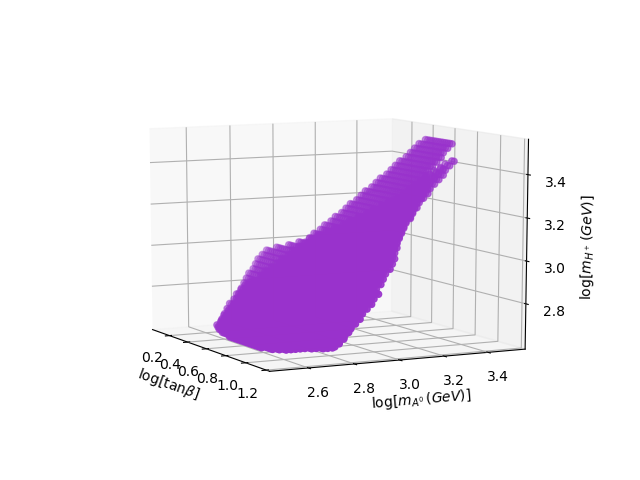
\includegraphics[width=0.6\textwidth,trim=6em 3em 10pt 6em,clip]{../global/threedimfit1.png}
    \caption{\label{fig:threed}Constraints in ($m_{H^+},m_{A^0},\tan\beta$) space from $B\to\mu^+\mu^-$ and the oblique parameters, where we assume $m_{A^0}\approx m_{H^0}$, and have scanned to $2\sigma$ in the alignment limit.
    The purple region indicates what is not excluded at 95\% CL.}
\end{figure}
Flavour constraints alone are not enough to give a full judgement on the 2HDM. 
There are other observables that can also provide indicative constraints on this model, such as the oblique parameters of the electroweak theory. 
These have not been the focus of this study, but we collaborate with \cite{james} for their work on the oblique parameters in the 2HDM (working from the expressions given in \cite{oblique,hunter}), and add these to the global 2HDM fit. 
These observables have a different dependency on the 2HDM parameters than the flavour observables considered here, depending on $\theta=\beta-\alpha$ rather than $\beta$, $\alpha$ separately, as well as $m_{H^0}$ and $m_{A^0}$. 
The choice of $\beta-\alpha$ is fixed by our choice either of the alignment limit or the wrong sign limit, and we will therefore expect no variation across $\tan\beta$ for these constraints. 
There is however still dependency on $m_{H^0}$ and $m_{A^0}$ to consider.
We previously fixed $m_{H^0}=1.5\,$TeV, where it minimised $\chi^2$ across the range of test values used. 
Due to the additional dependencies here, we perform a test three-dimensional scan across ($m_{H^+},m_{A^0},\tan\beta$) space, assuming $m_{A^0}\approx m_{H^0}$, for the oblique parameters and $B_q\to\mu^+\mu^-$ as these are the only observables to have this additional dependency. 
In Figure \ref{fig:threed}, we see that there is a close linear relationship between $m_{A^0}$ and $m_{H^+}$, particularly for higher values. 
The value of $m_{H^+}$ is tightly constrained to be of a similar mass to $m_{H^0}$ and $m_{A^0}$. 
\hspace{-8pt}\footnote{In the work of \cite{james}, it is found that there can be fine-tuned solutions away from this close confinement. However, these are for values of $\theta$ away from either the alignment or wrong sign limits we consider here.}
\hspace{-3pt}Within the range of test values considered previously for $m_{H^0}$, we still find that $\chi^2$ is minimised for $m_{H^0}=1.5\,$TeV, so we choose to work with $m_{H^0}=m_{A^0}=1.5\,$TeV and test the two-dimensional global fit using these fixed parameters. 
\begin{table}[ht]
    \centering
    \begin{tabular}{c|c|c}
        \hline\hline
        \textbf{Model:} & $\cos(\beta-\alpha)=\sin(2\beta)$ & $\cos(\beta-\alpha)=0$ \\ 
        \hline\hline
        $m_{H^+}$ (GeV) & & $>270$ \\
        $m_{A^0}$ (GeV) & & $>210$ \\
        $\tan\beta$ & & $0.42\to54.7$ \\
        \hline
        $\chi^2_{min}$ & & $8.19$ \\
        $\chi^2_\nu$ & & $0.58$ \\
        $\nu$ & & $14$ \\
        p-value & & $87.9\%$ \\
        \hline\hline
    \end{tabular}
    \caption{\label{tab:pthreed}Constraints and statistics for three-dimensional fit from $2\sigma$ scan in Figure \ref{fig:threed}. 
    The fits have been done in the exact wrong-sign limit and the exact alignment limit as shown, and setting the additional 2HDM parameter $M=750\,$GeV. 
    For $m_{H^+}$, $m_{A^0}$ and $\tan\beta$, the constraint from each model at 95\% CL are shown.
    The information from the $\chi^2$ fitting of each model is then shown.}
    \vspace{-20pt}
\end{table}

\section{Discussion}
\label{sec:discuss}
We now show in Figure \ref{fig:global} the results of our fit, for the flavour observables discussed alone, and also including the oblique parameters from \cite{james}.
This has been done both in the alignment and wrong sign limits. 
As marked in the figure, it was found by \cite{oliver} that the exact wrong sign limit can only be allowed for $\tan\beta\gtrapprox6$ at the $2\sigma$ level, which significantly reduces the allowed region in our parameter space. 
This limit has not been included when performing the fit here, but we take note of the limitations this imposes on our results.

It is important to have any calculations performed confirmed by another source such that they maintain credibility, and to this end, the flavour observables studied throughout have been cross-checked in \cite{tom} as part a larger collaboration, and close agreement between results thus far has been found, lending to the validity of the results we present here. 

It is worth noting that, as we had in Section \ref{subsec:fit}, the 2HDM is a decoupling theory, so as we simultaneously take $m_{H^+},m_{H^0},m_{A^0}\to\infty$, we will recover the Standard Model results for these processes.
In the case of observables that are in agreement with the Standard Model, tending these masses to infinity will lead to a good statistical fit, as we would have in a Standard Model fit of these. 
Working several orders of magnitudes above the mass scales of the Standard Model particles approximates this limit to infinity, so to test a physical, and observable, Two Higgs Doublet Model Type II which is significant against the Standard Model, it is of no use looking to such large scales so we therefore remain working with more relevant mass scales as chosen for $m_{H^0}$ and $m_{A^0}$.
This effect is also seen in the $\chi^2$ fitting in Tables \ref{tab:pthreed}, \ref{tab:pval1}, and \ref{tab:pval2}. 
The value of $m_{H^+}$ that minimises $\chi^2$ for flavour observables alone and fixed $m_{H^0}$ is $3200\,$GeV, and similarly for $m_{A^0}$ and $m_{H^+}$ in the three-dimensional global fit. 
These values are not representative of what would actually minimise $\chi^2$ across any value these parameters could take, but rather the minimum within the range chosen, where we do not scan any higher than $3200\,$GeV for any mass. 
Were we to scan higher than this, we would expect a similar result whereby the values of $m_{H^+}$ and $m_{A^0}$ which minimise $\chi^2$ would be the highest value scanned to, and so on to the decoupling limit of this model. 
\begin{figure}[ht]
    \centering
    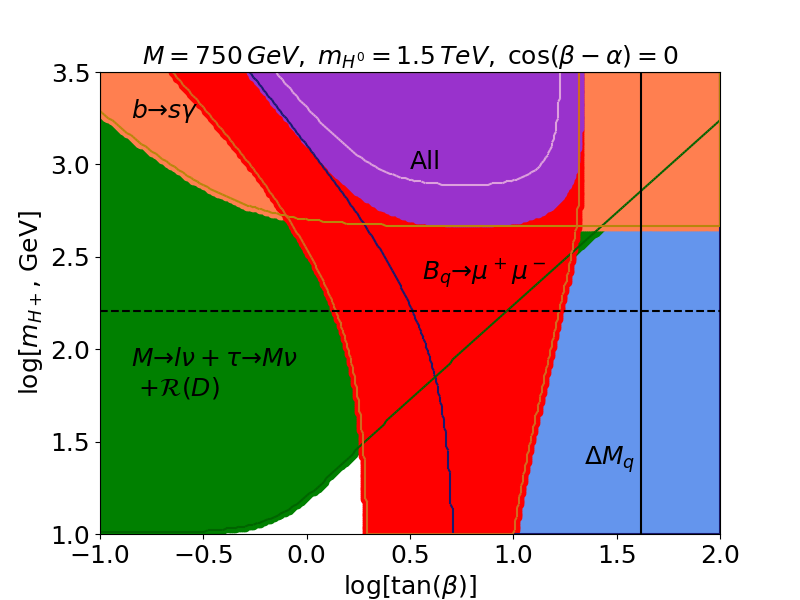
\includegraphics[width=0.49\textwidth]{../global/global_test.png}
    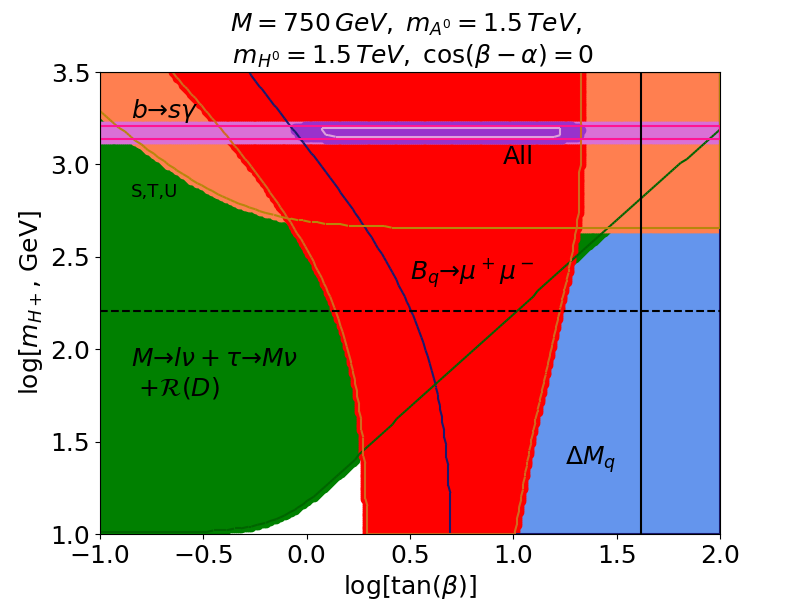
\includegraphics[width=0.49\textwidth]{../global/global_test2.png}
    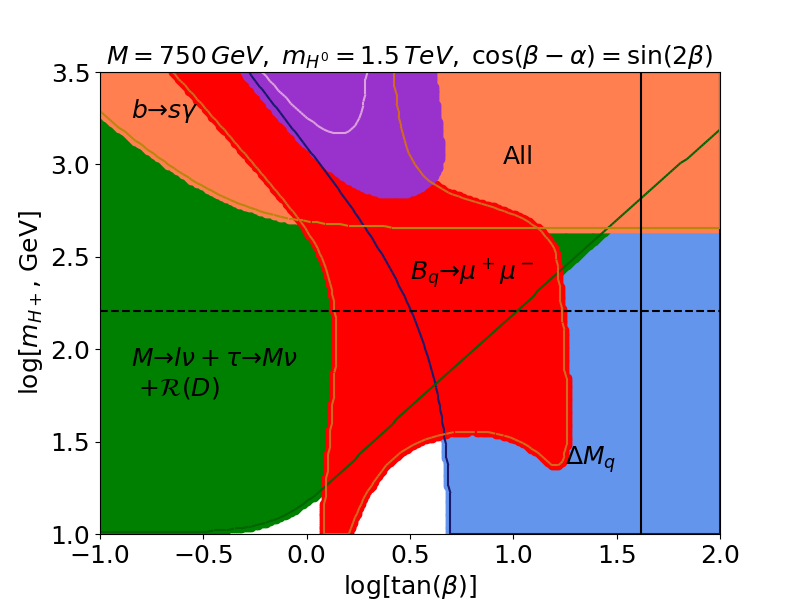
\includegraphics[width=0.49\textwidth]{../global/global_test5.png}
    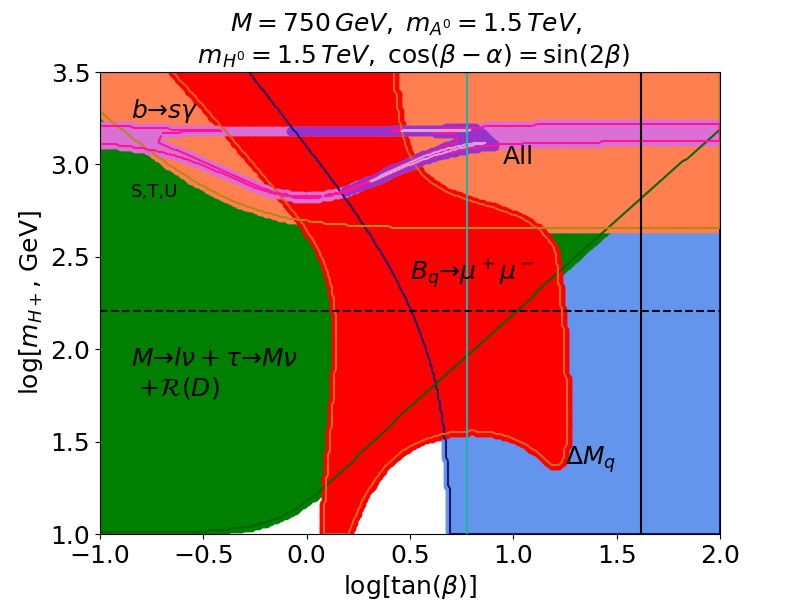
\includegraphics[width=0.49\textwidth]{../global/global_test6.png}
    \caption{\label{fig:global}Constraints on ($m_{H^+},\tan\beta$) in the alignment limit (top) and the wrong sign limit (bottom). 
    The constraints found in this work for flavour observables are shown (left), and then the oblique parameter constraints from \cite{james} are included too (right). 
    Each region shows what is not excluded for the relevant observables to 95\% CL as discussed in the text, then the line within the purple region for all observables marks out the $1\sigma$ confidence area. 
    The solid black vertical line shows $\tan\beta=m_t/m_b$, as for $\tan\beta$ much greater than this, the formulae for B mixing become invalid. 
    The dashed horizontal line marks the limit for a charged Higgs from direct searches, at $m_{H^+}>160\,$GeV \cite{dirhp}.
    For this two-dimensional fit, we fix the additional 2HDM parameters as in the titles of the plots and described in the text. 
    For the wrong sign limit, we use the exact form given in Eq. \ref{eq:wrongsign}, and mark with the vertical turquoise line the lower limit of its validity, as found by \cite{oliver}.
    The upper and lower bounds on parameters and the statistical indicators for each fit are shown in Table \ref{tab:pval1}.}
\end{figure}

We show in Table \ref{tab:pval1} the numerical constraints found in our parameter space from Figure \ref{fig:global}, and the statistical significance of the various fits. 
Due to the discrepancy found in $\mathcal{R}(D^*)$, different approaches were taken to explore its impact on the fit: in Table \ref{tab:pval1}, the statistical indicators for including this as an anomaly at $2\sigma$ are given, and then in brackets we give the indicators for a fit disregarding $\mathcal{R}(D^*)$ altogether, such that we see the impact this observable has on the validity of the 2HDM; we also show in Table \ref{tab:pval2} how the values of the constraints of our fit change for a $3\sigma$ scan as opposed to a $2\sigma$ scan, as at this error level, $\mathcal{R}(D^*)$ agrees with the shape of leptonic and semileptonic constraints, as shown in Figure \ref{fig:rd3sig}.
\begin{table}[ht]
    \centering
    \begin{tabular}{cc|C{1cm}C{1.1cm}|C{1cm}C{1.4cm}|C{1cm}C{1.2cm}|C{1.2cm}C{1.2cm}}
        \hline\hline
        \multicolumn{2}{c|}{\multirow{2}{*}{\textbf{Model:}}} & \multicolumn{4}{c}{$\cos(\beta-\alpha)=\sin(2\beta)$} & \multicolumn{4}{|c}{$\cos(\beta-\alpha)=0$} \\ 
        \cline{3-10}
        & & \multicolumn{2}{c|}{\textbf{Flavour}} & \multicolumn{2}{C{2.4cm}|}{\textbf{Flavour + Oblique}} & \multicolumn{2}{c|}{\textbf{Flavour}} & \multicolumn{2}{C{2.4cm}}{\textbf{Flavour + Oblique}} \\
        \hline\hline
        $m_{H^+}$: & 95\% CL & \multicolumn{2}{c|}{$>740$} & \multicolumn{2}{c|}{$720\to1580$} & \multicolumn{2}{c|}{$>480$} & \multicolumn{2}{c}{$1380\to1620$} \\
        (GeV)                & $1\sigma$ & \multicolumn{2}{c|}{$>1510$} & \multicolumn{2}{c|}{$790\to1540$} & \multicolumn{2}{c|}{$>750$} & \multicolumn{2}{c}{$1410\to1580$} \\
                         & $\chi^2_{min}$ & \multicolumn{2}{c|}{$3200$} & \multicolumn{2}{c|}{$1510$} & \multicolumn{2}{c|}{$3200$} & \multicolumn{2}{c}{$1440$} \\
        \hline
        $\tan\beta$: & 95\% CL & \multicolumn{2}{c|}{$<4.03$} & \multicolumn{2}{c|}{$0.84\to8.1$} & \multicolumn{2}{c|}{$<21.3$} & \multicolumn{2}{c}{$0.9\to21.3$} \\
                     & $1\sigma$ & \multicolumn{2}{c|}{$<1.92$} & \multicolumn{2}{c|}{$1.1\to7.9$} & \multicolumn{2}{c|}{$<17.3$} & \multicolumn{2}{c}{$1.2\to16.8$} \\
                     & $\chi^2_{min}$ & \multicolumn{2}{c|}{$0.98$} & \multicolumn{2}{c|}{$1.9$} & \multicolumn{2}{c|}{$4.1$} & \multicolumn{2}{c}{$5.2$} \\
        \hline
        \multicolumn{2}{c|}{$\chi^2_{min}$} & $20.6$ & ($11.5$) & $24.6$ & ($16.6$) & $18.1$ & ($9.78$) & $18.6$ & ($10.3$) \\
        \multicolumn{2}{c|}{$\chi^2_{\nu}$} & $1.7$ & ($1.0$) & $1.6$ & ($1.2$) & $1.5$ & ($0.9$) & $1.2$ & ($0.7$) \\
        \multicolumn{2}{c|}{$\nu$} & $12$ & ($11$) & $15$ & ($14$) & $12$ & ($11$) & $15$ & ($14$)\\
        \multicolumn{2}{c|}{p-value} & $5.7\%$ & ($40\%$) & $5.5\%$ & ($28\%$) & $11\%$ & ($55\%$) & $23\%$ & ($74\%$) \\
        \hline\hline
    \end{tabular}
    \caption{\label{tab:pval1}Constraints and statistics for global fits following $2\sigma$ scans. `Flavour' denotes all of the flavour observables discussed throughout, including $R(D^*)$ as an anomaly; `Oblique' denotes adding the three oblique parameters from \cite{james}. 
    The fits have been done in the exact wrong-sign limit and the exact alignment limit as shown, and setting the additional 2HDM parameters as $M=750\,$GeV and $m_{H^0}=m_{A^0}=1.5\,$TeV. 
    For $m_{H^+}$ and $\tan\beta$, the constraints from each model at 95\% CL and $1\sigma$ and their $\chi^2_{min}$ values are shown respectively.
    The information from the $\chi^2$ fitting of each model is then shown, first for the inclusion of the anomalous $\mathcal{R}(D^*)$ in this fit, and then in brackets we show the fit in we were to exclude $\mathcal{R}(D^*)$.
    The 2HDM potential parameter $M$ does not impact the fit as it varies, although through the oblique parameters, $m_{H^0}$ and $m_{A^0}$ will cause our results to vary as these require all new Higgs masses to be approximately equal, thus confining the space tightly near whatever values are chosen for these masses.
    The constraints, therefore, which include the oblique parameters are test constraints for fixed $m_{H^0}=m_{A^0}$ as above, and not indicative of global constraints. 
    The flavour alone constraints, however, do give a minimum constraint of $m_{H^+}$ with no extra dependency.}
\end{table}
The effect of $\mathcal{R}(D^*)$ at $2\sigma$ is clear. 
Including $\mathcal{R}(D^*)$ almost doubles $\chi^2_{min}$ in most of the cases shown, and heavily reduces the p-values for these fits, taking them from where we could still consider the 2HDM a valid hypothesis, to where we now near definite exclusion of this model (under the conditions imposed here).
We do not propose any further solution to the problem of $\mathcal{R}(D^*)$ here, though we recognise one must be found if the Two Higgs Doublet Model Type II could still be considered.
%REWORD

Due to the additional dependencies from the oblique parameters, we cannot conclude many limitations in our ($m_{H^+},\tan\beta$) parameter space, apart from that $H^+$ must have a similar mass to $H^0$ and $A^0$. 
The most definitive constraints on $m_{H^+}$ and $\tan\beta$ come from the $b\to s\gamma$ radiative decay and $B_q\to\mu^+\mu^-$ repectively. 
The flavour constraints in Table \ref{tab:pval1} show the minimum value for $m_{H^+}$ that is primarily constrained from $b\to s\gamma$, and also show the maximum $\tan\beta$ as constrained from $B_q\to\mu^+\mu^-$. 
This $\tan\beta$ constraint is, however, dependent on $m_{H^0}$, and is therefore not conclusive due to the lack of constraint on this parameter. 
The maximum allowed value for $\tan\beta$ is seen to increase with larger $m_{H^0}$, as shown in Figure \ref{fig:bmu}, and so, this is only indicative of the limitations for larger $\tan\beta$ for more finite masses as considered here.
\begin{itemize}
    \item $R(D^*)$ is a killer, Table demonstrates how significantly it changes the fit. Do not propose a solution for this here, but one must be found for any 2HDM to be valid. 
    \item P-values all very low, particularly when including $R(D^*)$ - likelihood of model being correct is very small
    \item Wrong sign limit fits worse than alignment limit - in WSL, obliques make fit worse, can see a strange pattern in its allowed region in the figure, discussed more in James' paper mayybe; in AL, obliques make fit betterm coming from theta dependence, less variation close to pi/2
    \item From 3d figure and table, expect fit to get better again as we increase fixed vals, but this is less significant against the SM - ramble on more about decoupling 
    \item WSL gets even more likely with Oliver's constraint - very slim space for tanb with obliques, but nothing at all for flavour alone - would expect more space for lower mH0 near the bsgamma limit
    \item AL still somewhat possible, but $R(D^*)$ kills it - main limit is still bsgamma then roughly equal masses
    \item Future works - inclusion of NLO mixing, add SM4 for full exclusion of SM4x2HDM in wrong sign limit, three/four/+ dimensional fits properly
\end{itemize}

\begin{table}[ht]
    \centering
    \begin{tabular}{cc|C{2.4cm}|C{2.2cm}|C{1.8cm}|C{2.4cm}}
        \hline\hline
        \multicolumn{2}{c|}{\multirow{2}{*}{\textbf{Model:}}} & \multicolumn{2}{c}{$\cos(\beta-\alpha)=\sin(2\beta)$} & \multicolumn{2}{|c}{$\cos(\beta-\alpha)=0$} \\ 
        \cline{3-6}
        & & \textbf{Flavour} & \textbf{Flavour + Oblique} & \textbf{Flavour} & \textbf{Flavour + Oblique} \\
        \hline\hline
        $m_{H^+}$ (GeV): & 95\% CL & $>740$ & $720\to1620$ & $>490$ & $1380\to1620$ \\
                         & $1\sigma$ & $>1510$ & $790\to1540$ & $>780$ & $1410\to1580$ \\
                         & $\chi^2_{min}$ & $3200$ & $1510$ & $3200$ & $1440$ \\
        \hline
        $\tan\beta$: & 95\% CL & $<4$ & $0.8\to32$ & $<21$ & $0.9\to21$ \\
                     & $1\sigma$ & $<1.9$ & $1.1\to7.7$ & $<17$ & $1.2\to17$ \\
                     & $\chi^2_{min}$ & $0.98$ & $1.9$ & $4.1$ & $5.2$ \\
        \hline
        \multicolumn{2}{c|}{$\chi^2_{min}$} & $20.6$ & $25.7$ & $18.8$ & $19.4$ \\
        \multicolumn{2}{c|}{$\chi^2_{\nu}$} & $1.71$ & $1.71$ & $1.57$ & $1.29$ \\
        \multicolumn{2}{c|}{$\nu$} & $12$ & $15$ & $12$ & $15$ \\
        \multicolumn{2}{c|}{p-value} & $5.7\%$ & $4.2\%$ & $9.3\%$ & $19.8\%$ \\
        \hline\hline
    \end{tabular}
    \caption{\label{tab:pval2}Constraints and statistics for global fits following $3\sigma$ scans. `Flavour' denotes all of the flavour observables discussed throughout, including $R(D^*)$ which fits to this level; `Oblique' denotes adding the three oblique parameters from \cite{james}. 
    The fits have been done in the exact wrong-sign limit and the exact alignment limit as shown, and setting the additional 2HDM parameters as $M=750\,$GeV and $m_{H^0}=m_{A^0}=1.5\,$TeV. 
    For $m_{H^+}$ and $\tan\beta$, the constraints from each model at 95\% CL and $1\sigma$ and their $\chi^2_{min}$ values are shown respectively.
    The information from the $\chi^2$ fitting of each model is then shown.
    The 2HDM potential parameter $M$ does not impact the fit as it varies, although through the oblique parameters, $m_{H^0}$ and $m_{A^0}$ cause our results to vary as these require all new Higgs masses to be approximately equal, thus confining the space tightly near whatever values are chosen for these masses.}
\end{table}

%\section{CKM Element Modification}

\section{Conclusion}

%\appendix
%\section{Some title}
%Please always give a title also for appendices.
%
%\acknowledgments
%This is the most common positions for acknowledgments. A macro is
%available to maintain the same layout and spelling of the heading.
%
%\paragraph{Note added.} This is also a good position for notes added
%after the paper has been written.

\begin{thebibliography}{99}

\bibitem{bail} %n gauge transforms
D. Bailin and A. Love, \emph{Introduction to Gauge Field Theory} (Institute of Physics, 1993).

\bibitem{schwartz} %o Higgs
M.D. Schwartz, \emph{Quantum Field Theory and the Standard Model} (Cambridge University Press, 2018).

\bibitem{kane} %m covar deriv
G. Kane, \emph{Modern Elementary Particle Physics} (Addison-Wesley, 1987).

\bibitem{lee}
T. Lee and C. Yang, \emph{Question of Parity Conservation in Weak Interactions}, Phys. Rev. \textbf{104} (1956) 254-258, doi:10:1103/PhysRev.104.254.

\bibitem{wu}
C. Wu et al, \emph{Experimental Test of Parity Conservation in $\beta$ Decay}, Phys. Rev. \textbf{105} (1957), 1413-1414, doi:10.1103/PhysRev.105.1413.

\bibitem{higgs}
P. W. Higgs, \emph{Broken Symmetries and the Masses of Gauge Bosons}, Phys. Rev. Lett. \textbf{13} (1964) 508-509, doi:10.1103/PhysRevLett.13.508.

\bibitem{dono} %l CKM ref
J.F. Donoghue, E. Golowich, and B.R. Holstein, \emph{Dynamics of the Standard Model} (Cambridge University Press, 2014).

\bibitem{pdg} %d
M. Tanabashi et al [Particle Data Group], Phys. Rev. D98, 030001 (2018) and 2019 update

\bibitem{wolf}
L. Wolfenstein, \emph{Parametrization of the Kobayashi-Maskawa Matrix}, Phys. Rev. Lett. \textbf{51} (1983), doi:10.1103/PhysRevLett.51.1945.

\bibitem{ckm} %g
CKMfitter Group (J. Charles et al.), Eur. Phys. J. C41, 1-131 (2005) [hep-ph/0406184], updated results and plots available at: \href{http://ckmfitter.in2p3.fr}{http://ckmfitter.in2p3.fr}.

\bibitem{sak} %h
A. Sakharov, \emph{Violation of CP Invariance, C asymmetry, and Baryon Asymmetry of the Universe}, Pisma Zh. Eksp. Teor. Fiz. 5 (1967) 32 [JETP Lett. 5 (1967) 24] [Sov. Phys. Usp. 34 (1991) 392] [Usp. Fiz. Nauk 161 (1991) 61].

\bibitem{sphal}
F. R. Klinkhamer and N. Manton, \emph{A Saddle Point in the Weinberg-Salam Theory}, Phys. Rev. D \textbf{30} (1984) 2212, doi:10.1103/PhysRevD.30.2212.

\bibitem{cpv}
J. Christenson et al, \emph{Evidence for the $2\pi$ Decay of the $K_2^0$ Meson}, Phys. Rev. Lett. \textbf{13} (1964), 138-140, doi:10.1103/PhysRevLett.13.138.

\bibitem{zp} %p
T.G. Rizzo, \emph{Z' Phenomenology and the LHC}, [\href{https://arxiv.org/abs/hep-ph/0610104}{arXiv:0610104 [hep-ph]}].

\bibitem{sm4} %r
A. Lenz, \emph{Constraints on a Fourth Generation of Fermions from Higgs Boson Searches}, Adv. High Energy Phys. \textbf{2013} (2013) 910275, doi:10.1155/2013/910275.

\bibitem{shal} %q
S. Bar-Shalom, M. Geller, S. Nandi, and A. Soni, \emph{Two Higgs doublets, a 4th generation and a 125 GeV Higgs: a review}, Adv. High Energy Phys. \textbf{2013} (2013) 672972, doi:10.1155/2013/672972, [\href{https://arxiv.org/abs/1208.3195v2}{arXiv:1208.3195 [hep-ph]}].

\bibitem{branco} %s
G.C. Branco et al, \emph{Theory and phenomenology of two-Higgs-doublet models}, Phys. Rept. \textbf{516} (2012) 1-102, doi:10.1016/j.physrep.2012.02.002, [\href{https://arxiv.org/pdf/1106.0034.pdf}{arXiv:1106.0034 [hep-ph]}].

\bibitem{desc} %a
O. Deschamps et al, \emph{The Two Higgs Doublet Model of Type II facing flavour physics data}, Phys. Rev. D \textbf{82} (2010) 073012, doi:10.1103/PhysRevD.82.073012, [\href{https://arxiv.org/abs/0907.5135}{arXiv:0907.5135 [hep-ph]}].

\bibitem{mix15}
M. Artuso, G. Borissov, and A. Lenz, \emph{CP Violation in the $B_s^0$ system,} Rev. Mod. Phys. \textbf{88} (2016) no.4 045002, doi:10.1103/RevModPhys.88.045002, [\href{https://arxiv.org/abs/1511.09466}{arXiv:1511.09466 [hep-ph]}].

\bibitem{bmix} %i
L. Di Luzio, M. Kirk, A. Lenz, and T. Rauh, \emph{$\Delta M_s$ theory precision confronts flavour anomalies}, JHEP \textbf{12} (2019) 009, doi:10.1007/JHEP12(2019)009, [\href{https://arxiv.org/abs/1909.11087}{arXiv:1909.11087 [hep-ph]}].

\bibitem{susy} %b
G. Degrassi, P. Gambino, and P. Slavich, \emph{SusyBSG: a fortran code for} BR$[B\to X_s\gamma]$ \emph{in the MSSM with Minimal Flavor Violation}, Comput. Phys. Commun. \textbf{179} (2008) 759-771, doi:10.1016/j.cpc.2008.06.012, [\href{https://arxiv.org/abs/0712.3265}{arXiv:0712.3265 [hep-ph]}].

\bibitem{bmes} %f
A. Lenz and G. Tetlalmatzi-Xolocotzi, \emph{Model-independent bounds on new physics effects in non-leptonic tree-level decays of B-mesons}, [\href{https://arxiv.org/abs/1912.07621}{arXiv:1912.07621 [hep-ph]}].

\bibitem{dirhp}
M. Aaboud et al [ATLAS], \emph{Search for charged Higgs bosons decaying via $H^{\pm}\to\tau^\pm\nu_\tau$ in the $\tau+$jets and $\tau+$lepton final states with $36\,$fb$^{-1}$ of $pp$ collision data recorded at $\sqrt{s}=14\,$TeV with the ATLAS experiment}, JHEP \textbf{09} (2018) 139, doi:10.1007/JHEP09(2018)139, [\href{https://arxiv.org/abs/1807.07915}{arXiv:1807.07915 [hep-ex]}].

\bibitem{bmu}
M. T. Prim et al [Belle Collaboration], \emph{Search for $B^+\to\mu^+\nu_\mu$ and $B^+\to\mu^+N$ with inclusive tagging}, Phys. Rev. D \textbf{101} (2020) no.3 032007, doi:10:1103/PhysRevD.101.032007, [\href{https://arxiv.org/abs/1911.03186}{arXiv:1911.03186 [hep-ex]}].

\bibitem{hflav} %c
Y. Amhis et al [HFLAV], \emph{Averages of b-hadron, c-hadron, and $\tau$-lepton properties as of 2018}, [\href{https://arxiv.org/abs/1909.12524}{arXiv:1909.12524 [hep-ex]}].

\bibitem{bxu} %e
A. Sibidanov et al [Belle], \emph{Study of Exclusive $B\to X_ul\nu$ Decays and Extraction of $|V_{ub}|$ using Full Reconstruction Tagging at the Belle Experiment}, Phys. Rev. D \textbf{88} (2013) no.3 032005, doi:10.1103.PhysRevD.88.032005, [\href{https://arxiv.org/abs/1306.2781}{arXiv:1306.2781 [hep-ex]}].

\bibitem{flag} %j
S. Aoki et al [FLAG], \emph{FLAG Review 2019}, Eur. Phys. J. C \textbf{80} (2020) no.2 113, doi:10.1140/epjc/s10052-019-7354-7, [\href{https://arxiv.org/abs/1902.08191}{arXiv:1902.08191 [hep-lat]}].

\bibitem{alex} %k
A. Lenz, private correspondence.

\bibitem{criv}
A. Crivellin, D. M\"{u}ller, and C. Wiegand, \emph{$b\to sl^+l^-$ transitions in two-Higgs-doublet models}, JHEP \textbf{06} (2019) 119, doi:10.1007/JHEP06(2019)119, [\href{https://arxiv.org/abs/1903.10440}{arXiv:1903.10440 [hep-ph]}].

\bibitem{lrgtb}
H. E. Logan and U. Nierste, \emph{$B_{s,d}\to l^+l^-$ in a two Higgs doublet model}, Nucl. Phys. B \textbf{586} (2000) 39-55, doi:10.1016/S0550-3213(00)00417-X, [\href{https://arxiv.org/abs/hep-ph/0004139}{arXiv:0004139 [hep-ph]}].

\bibitem{trilin}
P. Arnan, D. Be\v{c}irevi\v{c}, F. Mescia, and O. Sumensari, \emph{Two Higgs doublet models and $b\to s$ exclusive decays}, Eur. Phys. J. C \textbf{77} (2017) no.11 796, doi:10.1140/epjc/s10052-017-5370-z, [\href{https://arxiv.org/abs/1703.03426}{arXiv:1703.03426 [hep-ph]}].

\bibitem{h0search}
A. M. Sirunyan et al [CMS], \emph{Search for MSSM Higgs bosons decaying to $\mu^+\mu^-$ in proton-proton collisions at $s=13\,$TeV}, Phys. Lett. B \textbf{798} (2019) 134992, doi:10.1016/j.physletb.2019.134992, [\href{https://arxiv.org/abs/1907.03152}{arXiv:1907.03152 [hep-ex]}].

\bibitem{rds}
J. Lee, \emph{$B\to D^{(*)}\tau\nu_\tau$ in the 2HDM with an anomalous $\tau$ coupling}, Phys. Rev. D \textbf{96} (2017) no.5 055005, doi:10.1103/PhysRevD.96.055005, [\href{https://arxiv.org/abs/1705.02465}{arXiv:1705.02465 [hep-ph]}].

\bibitem{couple}
A. M. Sirunyan et al [CMS], \emph{Combined measurements of Higgs boson couplings in proton-proton collisions at $\sqrt{s}=13\,$TeV}, Eur. Phys. J. C \textbf{79}(2019) no.5 421, doi:10.1140/epjc/s10052-019-6909-y, [\href{https://arxiv.org/abs/1809.10733}{arXiv:1809.10733 [hep-ex]}].

\bibitem{wrong1}
D. Das, A. Kundu and I. Saha, \emph{Higgs data does not rule out a sequential fourth generation with an extended scalar sector}, Phys. Rev. D \textbf{97} (2018) no.1 011701, doi:10.1103/PhysRevD.97.011701, [\href{https://arxiv.org/abs/1707.03000}{arXiv:1707.03000 [hep-ph]}].

\bibitem{wrong2}
M. Raju, J. P. Saha, D. Das and A. Kundu, \emph{Double Higgs production as an exclusive probe for a sequential fourth generation with wrong-sign Yukawa couplings}, Phys. Rev. D \textbf{101} (2020) no.5 055036, doi:10.1103/PhysRevD.101.055036, [\href{https://arxiv.org/abs/2001.05280}{arXiv:2001.05280 [hep-ph]}].

\bibitem{oliver}
O. Atkinson, private correspondence.

\bibitem{james}
J. Wynne, private correspondence.

\bibitem{oblique}
W. Grimus, L. Lavoura, O. Ogreid and P. Osland, \emph{The Oblique parameters in multi-Higgs models}, Nucl. Phys. B \textbf{801} (2008) 81-96, doi:10.1016/j.nuclphysb.2008.04.019, [\href{https://arxiv.org/abs/0802.4353}{arXiv:0802.4353 [hep-ph]}].

\bibitem{hunter}
J. Gunion, H. Haber, G. Kane, and S. Dawson, \emph{The Higgs Hunter's Guide} (CRC Press, 2018).

\bibitem{tom}
T. Eaton, private correspondence.

\end{thebibliography}


\end{document}
